\documentclass[10pt]{article}
% \usepackage[margin=1in]{geometry}
% \newcommand\hmmax{0}
% \newcommand\bmmax{0}
% % % Fonts% %
% \usepackage{luatexja}

\usepackage[T1]{fontenc}
   % \usepackage{textcomp}
   % \usepackage{newtxtext}
   % \renewcommand\rmdefault{Pym} %\usepackage{mathptmx} %\usepackage{times}
\usepackage[complete, subscriptcorrection, slantedGreek, mtpfrak, mtpbb, mtpcal]{mtpro2}
   \usepackage{bm}% Access to bold math symbols
   % \usepackage[onlytext]{MinionPro}
   \usepackage[no-math]{fontspec}
   \defaultfontfeatures{Ligatures=TeX,Numbers={Proportional}}
   \newfontfeature{Microtype}{protrusion=default;expansion=default;}
   \setmainfont[Ligatures=TeX,BoldFont={*-Semibold}]{Source Serif Pro}
   \setsansfont[Microtype,Scale=MatchLowercase,Ligatures=TeX,BoldFont={*-Semibold}]{Source Sans Pro}
   \setmonofont[Scale=0.8]{Atlas Typewriter}
   % \usepackage{selnolig}% For suppressing certain typographic ligatures automatically
% % % % % % %
\usepackage{amsthm}         % (in part) For the defined environments
\usepackage{mathtools}      % Improves  on amsmaths/mtpro2
\usepackage{xfrac}

% % % The bibliography % % %
\usepackage[backend=biber,
  style=authoryear-comp,
  bibstyle=authoryear,
  citestyle=authoryear-comp,
  uniquename=false,
  % allinit,
  % giveninits=true,
  backref=false,
  hyperref=true,
  url=false,
  isbn=false,
  useprefix=true,
  ]{biblatex}
\DeclareFieldFormat{postnote}{#1}
\DeclareFieldFormat{multipostnote}{#1}
% \setlength\bibitemsep{1.5\itemsep}
\newcommand{\noopsort}[1]{}
\addbibresource{Thesis.bib}

% % % % % % % % % % % % % % %

\usepackage[inline]{enumitem}
\setlist[enumerate]{noitemsep}
\setlist[description]{style=unboxed,leftmargin=\parindent,labelindent=\parindent,font=\normalfont\space}
\setlist[itemize]{noitemsep}

% % % Misc packages % % %
\usepackage{setspace}
% \usepackage{refcheck} % Can be used for checking references
% \usepackage{lineno}   % For line numbers
% \usepackage{hyphenat} % For \hyp{} hyphenation command, and general hyphenation stuff

% % % % % % % % % % % % %

% % % Red Math % % %
\usepackage[usenames, dvipsnames]{xcolor}
% \usepackage{everysel}
% \EverySelectfont{\color{black}}
% \everymath{\color{red}}
% \everydisplay{\color{black}}
\definecolor{fuchsia}{HTML}{FE4164}%Neon Fuchsia %{F535AA}%Neon Pink
% % % % % % % % % %

\usepackage[export]{adjustbox}
\usepackage{subcaption}

% \usepackage{pifont}
% \newcommand{\hand}{\ding{43}}
\usepackage{array}


\usepackage{multirow}
% \usepackage{adjustbox}

\usepackage{titlesec}

\usepackage{multicol}

\setcounter{secnumdepth}{4}
\setcounter{tocdepth}{4}

\usepackage{tikz}
\usetikzlibrary{bending,arrows,positioning,calc}
\usetikzlibrary{arrows.meta}
\usepackage{tikz-qtree} %for simple tree syntax
% \usepgflibrary{arrows} %for arrow endings
% \usetikzlibrary{positioning,shapes.multipart} %for structured nodes
\usetikzlibrary{tikzmark}
\usetikzlibrary{patterns}

\usepackage{graphicx} % for images (png/jpeg etc.)
\usepackage{caption} % for \caption* command

\usepackage{tabularx}

\usepackage{bussalt}

\usepackage{Oblique} % Custom package for oblique commands
\usepackage{CustomTheorems}
\usepackage{FuturePromisedEvents}

% \usepackage{svg}
% \usepackage[off]{svg-extract}
% \svgsetup{clean=true}

\usepackage{dashrule}

\newcommand{\hozline}[0]{%
  \noindent\hdashrule[0.5ex][c]{\textwidth}{.1pt}{}
  %\vspace{-10pt}
  % \noindent\rule{\textwidth}{.1pt}
}

\newcommand{\hozlinedash}[0]{%
  \noindent\hdashrule[0.5ex][c]{\textwidth}{.1pt}{2.5pt}
  %\vspace{-10pt}
}

\usepackage{contour}
% \usepackage{pdfrender}

\usepackage{extarrows}

% % % My commands % % %

% % % % % % % % % % % %

\usepackage{xskak} % For chess diagram


\usepackage[hidelinks,breaklinks]{hyperref}

\title{Only take me as far as I can go by myself}
% \subtitle{\dots and you don't need me to tell you}
\author{Ben Sparkes}
% \date{ }


\begin{document}

\tableofcontents

\hozlinedash

\begin{itemize}
\item significant interest:
  \begin{enumerate}
  \item Involuntarism
  \item Weakness of will
  \end{enumerate}
\end{itemize}

\begin{note}
  The point about involuntarism can be held independently from the broader point that I want to make.
  For, this is about restricting the choices of an agent, rather than providing the agent with choices, roughly stated.
  Hence, lack of ability make block, but it does not follow from this that instance of abilities opens.
\end{note}

\begin{itemize}
\item Observation about the possibility of rewriting support for an attitude may also be motivated by remembering.
\item E.g.\ ``Do you remember \(\phi\)''.
  In some cases there is additional information, but in other cases this is nothing more than an issue of attribution.
  The pragmatics are complex, however.
  If you do remember \(\phi\), then you also remember \(\psi\), hence if you answer `yes' then I don't need to tell you about \(\psi\), etc.
\end{itemize}

\newpage

The main motivation here is the common use of the idea of responding to reasons.
In particular, there's \citeauthor{Lord:2018aa} and others who hold the identity these, or \citeauthor{Broome:2013aa} with enkrasia, \citeauthor{Hieronymi:2018aa} with considerations, and others.
Representationalism and dispositionalismn, roughly.
If the proposition is true, then there's pressure.

On the one hand, understanding of phenomena.
On the other, ways in which to understand reasons/the relationship that agent's have with reasons.


\begin{note}[Functional role/function]
  The function of the attitude is (in part) determined by the reasons for which it is held.
  Individuate attitudes by their functional role, but an attitudes functional role does not (completely) determine its function.
\end{note}

\begin{note}[Quick argument]
  Quick argument is that reasons require direct response of a kind.
  Though I think I need to say more about direct response for this to be of interest.
  \begin{itemize}
  \item Agent to hold \(A\) on the basis of \(R\) requires \(R\) to do some explanatory work.
  \item If agent does not directly respond to \(R\) then \(R\) does not do any explanatory work.
  \item Therefore, reason only if directly respond.
  \end{itemize}
  The basic idea is that without direct response there's no difference between the reason obtaining and the reason not obtaining, from the agent's point of view.
  In this sense, the argument is similar to those that could be made against certain forms of responding directly to reasons, etc.

  The response to this is that the second premise is false.
  But if this is the case then superveniece is false.
  So, I should use superveniece in the argument!

  And, the `insight' is that this is replaced by supervenience on mind + ability, roughly stated.
  The difficulty with ability is that this is not something that depends on the agent's mind, so to speak, because whether the agent is able to do something depends on how the world develops.

  Right, although the argument here is similar to the one used against Lord and co.\ it is not clear that it generalises.
  This is because I depend on the role of ability, and without this there is no argument.

  The argument against this, the one that suggests this is a framework issue, is that one may consider an agent's perception of their abilities to be sufficient.
\end{note}






\newpage

\maketitle

\section{Introduction}
\label{sec:introduction-1}

Argue against:
\begin{itemize}
\item\label{denied-claim} \emph{An agent may appeal to reasons in support of a conclusion only if the agent used those reasons in some reasoning that yielded the conclusion.}
\end{itemize}

Contrapositive seems clear.
If agent used reasons in reasoning, then they may appeal to those reasons in support of the conclusion.
May be challenged and so on, but here interested in when the agent is forming the conclusion.
Unless give a strong normative reading of may, there doesn't seem any way to object.
Would deny that the reasoning is any good, not that the agent can cite their own reasoning.

Instead, contrast \emph{may} with \emph{must}.

Perhaps constitutive of reasoning, but then talk of raesoning instead.

Sketch argument for the conditional.

\begin{enumerate}
\item\label{opp:sketch:1} If conditional is false, then it is possible there are cases in which an agent is unaware of how the conclusion is supported by favoured reasons.
\item\label{opp:sketch:2} If agent is unaware of how a conclusion is supported by reasons, then conclusion may not be supported by those reasons.
\item\label{opp:sketch:3} If conclusion may not be supported, then the conclusion is not supported (from the agent's perspective).
\end{enumerate}

So, the agent may do as they please, but they will fail to establish support, the appeal would be in name only.

Contraposing and re-expressing, the last proposition, reads:

\begin{itemize}
\item If conclusion is supported by reasons, then it is a fact that the conclusion is supported by reasons.
\end{itemize}

Variation on a familiar thought that reasons are factive.\nolinebreak
\footnote{
  For example, \textcite[673]{Cunningham:2020aa}, summarising \textcite{Hornsby:2007aa,Hornsby:2007ab,Hornsby:2008aa} defends:
  \begin{quote}
    Necessarily, if S \(\phi\)'s because p then S knows that p
  \end{quote}
  Where the `because' is a rationalising `because'.
  If \emph{S} knows that \emph{p}, it is a fact that \emph{p}.
}
Here, relation of support is factive.

I think the last premise is more-or-less true, depending on how `may' is understood.
Perhaps the agent does not \emph{know} that the conclusion follows from the premises, but is \emph{confident} that the conclusion follows from the premises --- it would be bizarre if were not a fact that the conclusion is not supported by the premises.
Even so, it seems intuitive that an agent could not have the appropriate confidence without being away of how the conclusion is supported by the premises, and so some variation of \ref{opp:sketch:2} holds.
It seems plausible at least some variation of \ref{opp:sketch:1}--\ref{opp:sketch:3} is sound.\nolinebreak
\footnote{
  Alternative may be to argue for representationalism, or dispositionalism.
  \citeauthor{Neta:2019aa} for example of how these would go.
  Broad, and don't seem quite as informative.
}

I do not think some variation of \ref{opp:sketch:2} holds.
I think an agent may be unaware of how a conclusion is supported by reasons while the conclusion is supported by those reasons (from the agent's perspective and so on).

Focus is on a particular type of ability claim.
For example:
\begin{itemize}
\item ???
\end{itemize}

Argue for reading this as providing an agent with a \emph{license} to appeal to the reasoning (or reasons) that the agent is able to do.

Licenses recast a problem raised by \citeauthor{Davidson:2001aa}:
When we look to explain why an agent performed an act (here, adopting a conclusion), we find there are various account that \emph{could} explain.
(\citeauthor[7--8]{Davidson:2001aa})
\begin{quote}
  But then something essential has certainly been left out, for a person can have a reason for an action, and perform the action, and yet this reason not be the reason why they did it.
  Central to the relation between a reason and an action it explains is the idea that the agent performed the action \emph{because} they had the reason.\nolinebreak
  \mbox{}\hfill\mbox{(\citeyear[9]{Davidson:2001aa})}
\end{quote}
As \citeauthor{Hieronymi:2011aa} expresses, we seek `an explanation which shows, not merely what, from another’s point of view, \emph{could} count in favour of acting, but why that person did, in fact, act' (\citeyear[417]{Hieronymi:2011aa}).

Following \citeauthor{Davidson:2001aa}, then, reasons or reasoning only explain an action provided there is a causal relation between the reasons the agent had or the reasoning the agent performed, and the action.\nolinebreak
\footnote{
  Note on the inclusion of reasoning here.
  Later \citeauthor{Davidson:2001aa}: `I do not see how the right sort of causal process can be distinguished without, among other things, giving an account of how a decision is reached\dots' (\citeyear[232]{Davidson:2001aa}), etc.
  And, my focus.
}
If this is sound, then the difference between what \emph{could} explain and what \emph{does} explain is only a matter of what happened --- a causal relation does not distinguish explanation from non-explanation, but actual explanation from potential explanation.\nolinebreak
\footnote{
  In \citeauthor{Hieronymi:2011aa}'s phrasing: Without a causal relation we get an answer to ‘from so-and-so’s point of view, why do so such and such?’ rather than ‘why did so-and-so do such-and-such?’ (\citeyear[417]{Hieronymi:2011aa}).
}\(^{,}\)\nolinebreak
\footnote{
  {
    \color{red}
    This is different to the relationship that \citeauthor{Neta:2019aa} notes between reasons why and reasons for which.
    In short, reasons why are not always reasons for which, because there are explanatory relations which are in a sense `structural' and therefore are not seen as reasons from the agent's point of view.
    So, I'm colourblind, but that is not a reason for which I believe the two different colours are the same colour, though it explains why.
    Rather, the reasons for which is that both objects appear the same colour to me.

    The distinction I am interested in can be seen as distinction between the way a reason \emph{which} may support an attitude.
  }
}

Even if causal relations to not resolve the problem of distinguishing what could explain from what does explain, I take this problem to be genuine.
There is often no unique explanation for an action, potential explanations \emph{do} explain, but (merely) potential explanations do not explain what actually happened.
Yet, if potential explanations do explain, and an agent has a guarantee that a potential explanation obtains, then the agent has the guarantee of an explanation.

One does not need the theoretical backing to observe that the integer expression of \(7^{3}\) may be obtained by either mental arithmetic or a calculator.
And that if one is confident in their ability to perform mental arithmetic, then the use of the calculator demonstrates what they would obtain by performing the reasoning.
So, if one is provided with the information that one has the ability to perform the mental arithmetic to see that \(7^{3} = 343\), or that the calculator will show \(343\) after typing \(7^{3}\) in and hitting enter, it seems that either of these potential explanations may be cited as the explanation for holding that \(7^{3}\) is \(343\).

What explains why I hold that \(7^{3}\) is \(343\) is that the calculator would demonstrate that it is so, or \dots is that I have the ability to demonstrate that it is so.
The information provides only states that \(7^{3} = 343\) is the result of some process, and so I take that process to support holding that \(7^{3} = 343\).

{
  \color{red}
  The \citeauthor{Davidson:1963aa} motivation is quite general.
  I end up focusing on a particular case, where there are additional constraints to draw on.
  However, the result is of this kind, and I take this to be partial motivation for the possibility of these cases even when the additional constraints do not apply.

  Even so, role of ability in reasoning is interesting, and an instance of this type of thing.
}


\begin{note}[Fine distinction]
  The fine distinction is between an agent responding to reasons and an agent's action being supported by reasons.
  {
    \color{red}
    \emph{This!!!}
  }
  It is important to distinguish between the state of the board and the rules of chess, which are sufficient to derive the particular reasons, from this specific reason for which the move is possible.
  That it is a knight, knights can move, etc.
\end{note}

\hozlinedash





That an agent is able to reason may not be necessary, but helps with the explanation being potential --- a helpful divide between potential explanations and hypothetical explanations, perhaps.
Sufficient, at least.
Necessary and sufficient conditions aren't of interest.


Causal relations may not be correct.
Well, seems must not be correct.
This only goes part of the way.

Potential seems redundant.
Section ???










Here, agent obtains a license to a potential explanation.
Information about ability provides the agent with the information that the explanation could hold explain, or could stand in the appropriate causal relation.
Hence the agent performs the action `because' of the reasons or reasoning that would be invoked in the potential explanation.

{
\color{red} This skips over some details, esp.\ about how reasons/potential explanations are under-specified.
}

If the thing licensed isn't a potential explainer, then the agent would not have the ability, etc.\

Problem tasked with as theoreticians --- identifying the explanation --- is, in a sense, exploited by the agent given certain conditions.

Straightforward incompataibility.
Yes.
But only if assume (or demand) that the causal explanation is complete\dots




{
  \color{red}
  First part of the paper is walking through this carefully.
}
The upshot of denying~\ref{denied-claim} is flexibility in understanding agency.
Isolating, illustrating.



An important feature is that in the cases of interest, the conclusion does depend on reasoning to be true.
Some cases fail.
For example, agent cannot conclude that they have reasoned to the conclusion.
As, it is only the case that the agent has reasoned to the conclusion if the agent has performed the reasoning.
Reflexive content is often a source of trouble, but here the problem is more mundane.
An agent cannot turn on a light by reflecting on their ability, the agent must flick the switch in order for the light to turn on --- and reflexively referencing one's own reasoning requires a similar witnessing event.



Reasoning is great for various things other than obtaining a conclusion.
Agent goes with licensed reasons, they do not get this stuff.
However, the agent does get other things.





\hozlinedash

\section{Potential strategies}
\label{sec:potential-strategies}

\begin{note}[Narrowing cases]
  The motivating idea behind licensing is broad.
  It applies to any situation in which an agent is confident that a potential explanation is available.

  However, the argument for licensing is narrow.
  Look to specific cases.

  In the same way that there may be multiple potential explanations available to the agent, there may be multiple accounts to us as theorists.

  If an account can be given that does not involve licensing (or that do not involve the idea of licensing as anything other than a mistake), then the test is whether licensing is a best account.

  Assume that an account can be given that does not involve licensing.
  I doubt that it is possible to show that any given account is necessary.
  However, whether or not an account is best is not determined by the particular case.
  Depends also on the role of the account in other cases.
  Secure licensing in particular cases provides some support over alternatives when there is competition.\nolinebreak
  \footnote{
    Maybe a note here about the principle of charity.
    This is, I think, also a Davidsonian idea.
    Charity in the sense that one assumes that there is a rationalisation --- a (complete) explanation --- available.

    Charity, assume that if an agent's action is the result of reasoning then it may be rationalised --- in the sense of providing a complete explanation.
    Even a poor, but complete, explanation is preferable to an incomplete explanation (and hence absence of rationalisation).

    % May motivate with ideal cases.
    % Ideal cases seem to include possession of an explanation.
    % Soften the ideal by relaxing standards governing the quality of the explanation, rather than the existence of an explanation.
    % A poor explanation remains an explanation; potential explanation is only a \emph{potential} explanation.

  Corollary is the denial of this ordering on explanations.
  Sometimes appeal to a potential/incomplete explanation is better than a complete explanation.

  Conflicts with charity only if explanation is understood as complete explanation.
  Hence, I do not think that this conflicts with the spirit of charity, though it may conflict with particular accounts of charity.
  }

  This is about theory of explanations/reasons/reasoning.

  This limits attention.
  May be that licensing is rarely a best account.
  However, so long as it is a contender, then the main goal has been achieved.
\end{note}

\begin{note}[Outline of section]
  The goal of this section is to isolate a particular pattern of reasoning:
  \begin{enumerate}
  \item Information that agent possesses ability to reason \(\phi\).
  \item Endorsement of ability (not simply testimony).
  \item `Factive' inference to \(\phi\) being the case.
  \end{enumerate}
  Key piece of this reasoning is:
  \begin{itemize}
  \item Agent has the ability to \(\phi\) only if \(\phi\) is the case.
  \end{itemize}
  This is a necessary condition on the agent possessing the ability.
  Therefore, \emph{that} the agent possesses the ability can not be used to support \emph{that} \(\phi\) is the case.
  For the agent must already implicitly assume that \(\phi\) is the case.

  That the agent is informed is straightforward.
  The agent may avoid endorsing the ability, but this leads to some unnatural/indirect inference regarding assertion.
  Hence, endorsement of ability seems a plausible line of reasoning.

  Restructuring, I need to file some problems with ability inferences prior to working through testimony.

  In short, the problem is that there is no certainty with ability when the proposition is novel.
  For, the ability concerns a particular event type, bounded to the agent's current state.
  And as the agent has not yet witnessed their ability, at most one can obtain a high degree of confidence.

  So, rewriting the information, one obtains:
  \begin{itemize}
  \item I am confident that you have the ability to demonstrate that \dots
  \end{itemize}

  This is a subjective evaluation.
  Given the information the informer has, the have this degree of confidence.

  So, as the agent and the informer may have difference information, the agent needs to also endorse.

  For example, you may know that you do not understand how knights move.
  The informer seems fine with the confidence that they have --- they've seen you work through a number of puzzles and the absence of any knight move was not particularly noticeable, but this has been weighing on your mind.

  Hence, something along these lines shows the need for additional endorsement on the part of the agent.

  {
    \color{red}
    This may not be true in all cases of ability.
    For example, coach telling an athlete that they are able to perform a particular routine.
    Here, the coach may be an authority.

    Same may be true in some cases of reasoning, though this is trickier, due to lack of certainty.
    Rule following, etc.
    But then it seems that perhaps both the agent and the informer would be unsure, and it would remain the case that the informer could still be in a position of authority.
    Hence, narrower claim.

    This is about comparative positions, then.

    {
      \color{green}
      \emph{Wait!!!}
      This is optional.
      The role of the antecedent is to ensure that the agent needs to do some endorsement of their own.
    }
  }

  However, with the requirement of some endorsement in hand, the agent can not support \(\phi\) being the case.
  This holds even for \emph{confidence} that \(\phi\) is the case, as the relation of support is constrained.

  So, this pushes for either licensing or no inference.
  An additional point to make here is that this is not the \emph{only} motivation for licensing.
  For, there is also the difference between preservation of a designated value and construction of a witness.
  So, this forms a pair of a necessary and a sufficient observation.

  So, either the agent does not have support, or the support is licensed.

  There's no straightforward argument that the agent has (licensed) support.
  Idealised agents aren't to useful here, as we may assume that the ability will be witnessed.
  For agents like us, however, it seems we can use ability in reasoning.
  Though it is risky.

\end{note}

Consider the following:
\begin{enumerate}
\item\label{chess:claim:1} You are able to reason from the rules of chess and the game state (described in figure~\ref{fig:chess:board}) to the proposition that White cannot prevent Black from occupying c4 on their (Black's) second move.
\end{enumerate}
I assume claim~\ref{chess:claim:1} is true, but not immediately obvious.
And, in particular, that some reasoning from the rules of chess and the game state is required to verify the truth of the highlighted proposition.

For, in order to show that White cannot prevent Black from occupying c4 on their second move, you need to consider the moves that would be possible for Black on their second turn given the move that White made on their first turn in response to the move that Black made on their first turn, and so on.

\begin{note}[Confidence/Ability]
  I \emph{assume} that the statement is true.

  And, true because there's some potential future in which you have demonstrated, given the abilities that you currently possess.

  The statement may be false.
  So long as you have not performed the reasoning, I can not be sure.

  Subjective and objective uncertainty.
  Here, take it for granted that subjective.

  Statement about what could be.
  Future may not be determined, but potential futures.
  A little uneasy, but at the very least the subjective clouds out the objective.
  If ability statements are sometimes true, then there is some way of dealing with the objective component.

  \begin{enumerate}
  \item Informer is confident that agent has the ability.
  \item The informer's confidence is tied to the information available to the informer.
  \item The informer does not, in general, have a superior position.
  \item It is therefore up to the agent to endorse the informant's position.
  \item Seems, however, that there is in general something that the agent has access to that the informer does not.
  \item 
  \item The informer's statement depends on the information available to the informer.
  \item The informer's statement is made contingent on the information available to the informer.
  \item Some of the information is about what the agent is able to do.
  \item The informer's standpoint is inferior to the agent's standpoint with respect to this information.
    \begin{itemize}
    \item If the agent were to signal otherwise, then barring confusions, the informer would revise their assessment.
    \end{itemize}
  \item
  \item Therefore, the agent does not assert that the agent has the ability.
  \end{enumerate}
\end{note}

\begin{figure}[h]
  \centering
  \mbox{ }
  \hfill
  \begin{subfigure}{.4\textwidth}
    \begin{adjustbox}{minipage=\linewidth,scale=0.7}
      \centering
      \newchessgame[
      setwhite={ka5,pa3,pb4,pc4,pe5,pf6,bg5,bh5}, %{rc1,kh1,pa2,pb2,ph2,pf6,pg6,nc7,qf7},
      addblack={pa6,pb7,pc6,pe6,pf7,kc7,nd7,nd4}, %{rg2,pb5,pe5,qd6,pa7,pb7,ra8,bc8,kd8,bf8},
      ]%
      \setchessboard{showmover=false}%
      \chessboard
    \end{adjustbox}
    \caption{
      Game state\newline
      \mbox{ }\newline
    }
    \label{fig:chess:board}
  \end{subfigure}
  \mbox{ }
  \hfill
  \mbox{ }
  \begin{subfigure}{.4\textwidth}
    \begin{adjustbox}{minipage=\linewidth,scale=0.7}
      \centering
      \newchessgame[
      setwhite={ka5,pa3,pb4,pc4,pe5,pf6,bg5,bh5}, %{rc1,kh1,pa2,pb2,ph2,pf6,pg6,nc7,qf7},
      addblack={pa6,pb7,pc6,pe6,pf7,kc7,nd7,nd4}, %{rg2,pb5,pe5,qd6,pa7,pb7,ra8,bc8,kd8,bf8},
      ]%
      \setchessboard{showmover=false}%
      \chessboard[
      arrow=latex,
      linewidth=1pt,
      shortenstart=.8ex,
      shortenend=.5ex,
      pgfstyle=straightmove,
      strokeopacity=0.4,
      fillopacity=0.4,
      color=black,
      pgfstyle=border,
      markfields={c4,a3,a5,g6,c5},
      % markmoves={b7-b6,c6-c5,d4-c2,d4-b5,d4-f5,d4-e2,d4-f3,d4-b3,d7-c5,d7-b6,d7-b8,d7-f8,d7-f6,d7-e5,d7-e5,c7-c8,c7-b8,c7-d8,c7-b6,c7-d6}%{f7-g8,f7-e6,f7-d5,f7-c4,f7-b3,f7-e8,c7-d5,c7-b5,c7-a8,c7-e8,g6-g7,a2-a3,b2-b3,c1-a1,c1-b1,c1-d1,c1-e1,c1-f1,c1-g1,h2-h3,h1-g1,c1-c2,c1-c3,c1-c4,c1-c5,c1-c6}
      ]
    \end{adjustbox}
    \caption{Example fields White cannot prevent Black from occupying after two moves.}
    \label{fig:chess:move}
  \end{subfigure}
  \hfill
  \mbox{ }
  \caption{Black to checkmate in four moves.\protect\footnotemark}
  \label{fig:chess}
\end{figure}
\footnotetext{
  Puzzle 150 of \citeauthor{Emms:2000aa} (\citeyear[33]{Emms:2000aa}).
  \citeauthor{Emms:2000aa} provides the following solution:
  \begin{quote}
    \variation{1... Nb6!}
    (threatening \variation{2... Nb3\#})
    \variation{2. b5}
    (or \variation{2. Bd1 Nxc4+} \variation{3. Ka4 b5\#})
    \variation{2... c5!}
    \variation{3. bxa6 Nxc4+}
    \variation{4. Ka4 b5\#}
    \textbf{(0-1)}\nolinebreak
    \mbox{}
    \hfill
    (\citeyear[46]{Emms:2000aa})
  \end{quote}
}

To illustrate, Black may move the pawn from b7 to b5 on their first turn, and so be in a position to capture White's pawn on c4 in their second turn.
However, White may then prevent Black from occupying c4 on their next turn by using their pawn on c4 to capture Black's pawn on b5.
So, Black moving their pawn from b7 to b5 on their first turn is not an initial move of interest.

Still, there are only (a little more than) a handful of alternative moves and countermoves to consider, and so I not only assume that claim~\ref{chess:claim:1} is true, but I also assume that you also hold claim~\ref{chess:claim:1} to be true.
Even if you do not have an effective method for identifying a strategy for Black, you are able to exhaust all the strategies available to Black and identify those which ensure c5 is occupied on Black's second move.

Precisely, I assume that you hold claim~\ref{chess:claim:1} to be true at some interval between the point at which I claimed~\ref{chess:claim:1} is true and the present time or the point at which you demonstrated claim~\ref{chess:claim:1} to be true.\nolinebreak
\footnote{
  If a fresh instance of claim~\ref{chess:claim:1} is desired, one may substitute (e.g.) `a3', `a5', `g6', or `c5' for `c4'.
}
For ease of exposition, I will adopt the perspective of some point in that interval.
Therefore:
\begin{enumerate}[resume]
\item\label{chess:claim:2} White cannot prevent Black from occupying c4 on their second move.
% \item\label{chess:claim:3} You hold claim~\ref{chess:claim:2} to be true.
\item\label{chess:claim:4} You have not reasoned from the rules of chess and the game state (described in figure~\ref{fig:chess:board}) to \ref{chess:claim:2}. And,
\item\label{chess:claim:5} You hold that you are able to reason from the rules of chess and the game state to the truth of \ref{chess:claim:2}.
\end{enumerate}

Claim~\ref{chess:claim:5} is the result of holding claim~\ref{chess:claim:1} to be true, and claim~\ref{chess:claim:4} is true by assumption.

Further, claim~\ref{chess:claim:4} ensures that, as you have not reasoned from the rules of chess and the game state to \ref{chess:claim:2}, you do not hold claim~\ref{chess:claim:2} to be true due to a particular strategy that Black can enact.
Additionally, an account of why you hold claim \ref{chess:claim:2} is true does not follow from understanding the rules of chess and the game state alone.
For, an agent may understand the rules of chess and the game state while lacking the ability to demonstrate that claim~\ref{chess:claim:2} is true --- understanding the rules of chess and the game board is distinct from the ability to construct strategies.\nolinebreak
\footnote{
  Here I am relying on a principle \emph{like}:
  \begin{itemize}
  \item An agent's grasp of \(\Sigma\) can provide an account of why they hold \(\phi\) is true only if the agent has the ability to demonstrate that \(\phi\) follows from \(\Sigma\).
  \end{itemize}
  {
    \color{red}
    Whether or not this claim is true depends in part of how ability is understood\dots
  }

  Perhaps it is the case that claim~\ref{chess:claim:2} is sufficiently obvious to guarantee that the agent has the ability.
  Still, the reasoning involved differs only in complexity from the reasoning involved in showing that White cannot prevent Black from checkmating in four moves, and I doubt that this claim is sufficiently obvious.
}

Claim~\ref{chess:claim:2} follows from claim~\ref{chess:claim:1}.
For, if you are able to reason from the rules of chess and the game state to the proposition that White cannot prevent Black from occupying c4 on their second move, then \ref{chess:claim:2} must be true --- White cannot prevent Black from occupying c4 on their second move.
If White could prevent Black from occupying c4 on their second move, then you would not be able to reason from the rules of chess and the game state to an incompatible proposition.

My claim is important, given claim~\ref{chess:claim:4}.
However, the are (at least) two ways in which my claim relates to why you hold claim \ref{chess:claim:2} to be true.

First is testimony as a reason, roughly.
Extend the line of reasoning above.
You have my testimony that claim~\ref{chess:claim:1} is true, and claim~\ref{chess:claim:2} must be true if claim~\ref{chess:claim:1} is true, as noted above.

Colloquially, you may cite my testimony that claim~\ref{chess:claim:1} is true as support for holding that claim~\ref{chess:claim:2} is true.

{
  \color{red}
  \emph{Important!!!}
  I should be able to recast this without making use of the ability.
  For, there is a precondition on ability which is that the proposition is true.
  Hence, it seems as though one should be able to get to the conclusion without relying on the fact that one is able to do the reasoning.
  Though, this is tricky.
  The difference is between two conditionals.
  First, is ability entailing conclusion.
  Then second, is attribution of ability entailing conclusion.
  (I.e.\ it's something like a precondition of you even asserting that I am able as truthful that the conclusion holds, whether or not you are correct in your assertion.)
}

Note, however, that the entailment from claim~\ref{chess:claim:1} to claim~\ref{chess:claim:2} holds only if you are able to reason from the rules of chess and the game board to a strategy.

If you are not able to reason from the rules of chess and the game state, then claim~\ref{chess:claim:1} does not entail that White cannot prevent Black from occupying c4 on their second move.
It may be the case that White cannot prevent Black from occupying c4 on their second move and you are not able to figure this out, or it may be the case that White can prevent Black from occupying c4 on their second move.\nolinebreak
\footnote{
  % Pragmatics may suggest otherwise.
  It may be plausible to understand claim~\ref{chess:claim:1} as conveying additional information.
  For example:
  \begin{itemize}
  % \item You have the ability to demonstrate (the truth fact independent of your ability) that White can prevent Black from occupying c4 on their second move, or perhaps:
  \item White can prevent Black from occupying c4 on their second move \emph{and} you have the ability to demonstrate the former conjunct.
  \end{itemize}
  For, it is plausible to assume that I have identified a strategy, and the basis of my claim is my recognition that you are able to perform analogous reasoning.
  This is indeed the case for the present example.
  Therefore, you may infer that Black has a strategy regardless of ability.

  Two observations:
  \begin{enumerate*}[label=(\roman*)]
  \item Reasoning of this kind does not rule out the alternative line of reasoning that is of interest.
  \item The example may be made more complex. You claim that you have the ability to demonstrate that \(\phi\) follows from \(\Sigma\), and I have demonstrated that \(\psi\) follows from \(\phi\). I now claim that you are able to demonstrate that \(\psi\) follows from \(\Sigma\), as my reasoning was fairly simple, but I have not shown that \(\psi\) follows from \(\Sigma\), and therefore it would be a mistake to infer that I have stated that \(\psi\) follows from \(\Sigma\).
  \end{enumerate*}
  % However, it may also be the case that I have made a mistake, and therefore if you do not have the ability, then White can prevent Black from occupying c4 on their second move.

  % Complicating the example may avoid this problem.
  % For example, my goal is to indirectly demonstrate to you that you endorse and unsound inference.
}

So, if you hold it to be true that White cannot prevent Black from occupying c4 on their second move, you must also hold it to be true that you are able to reason from the rules of chess and the game state to a witnessing strategy for Black.
If you were to do the reasoning you are able to do, you would demonstrate a witnessing strategy for Black on the basis of the rules of chess and the game state.
And, if you were to demonstrate a witnessing strategy for Black on the basis of the rules of chess and the game state, you would not need to appeal to my testimony in order to hold that it to be true that White cannot prevent Black from occupying c4 on their second move.

Hence, in order for claim~\ref{chess:claim:1} to entail claim~\ref{chess:claim:2}, it must be the case that you are able to establish that claim~\ref{chess:claim:2} is true without appealing to my testimony.
In this way, claim~\ref{chess:claim:1} may be understood as guaranteeing a relation between your ability to reason from the rules of chess and the game state to the truth of a certain proposition.

Still, even though you would be able to demonstrate claim~\ref{chess:claim:2} without my testimony, my claim remains important in order for you to be confident that you have the ability --- even if you are confident that you understand the rules of chess and the game board, you would not be able to establish that White cannot prevent Black from occupying c4 on their second move without demonstrating a strategy for Black.
Claim~\ref{chess:claim:1} licenses you to hold that claim~\ref{chess:claim:2} is true on grounds that are independent of my testimony.

Colloquially, you may cite the reasoning that you are able to do (or the strategy that would result from the reasoning) as support for holding that claim~\ref{chess:claim:2} is true.
And my testimony that claim~\ref{chess:claim:1} is true is then cited in support of your ability to do the reasoning.\nolinebreak
\footnote{
  Similar phenomena with `do you also hold \(\phi\) to be true?'
  Well, you hold \(\phi\) to be true, etc.
  So on the basis of you asking this, I may hold \(\phi\) to be true.

  Or, may reason to \(\phi\).
  So, alternative paths is not unique to ability attributions, though this differs in an important way, as you do not gain from this confidence that you can demonstrate that \(\phi\) is the case independently of the interaction.
}

\begin{note}[The agent doesn't need to do anything]
  The third alternative is that the agent doesn't form an attitude, or does not form an attitude that commits the agent to the existence of a winning strategy.
  Agent may doubt the presuppositions hold, or may doubt that they have the ability.

  The agent has the option of committing to the existence of a winning strategy.
\end{note}

\begin{note}[Alertnative w/ programming]
  Modify the scenario a little.
  Written a program that does the reasoning, fairly explicit, in the terms that one would use.
  Certainly able to do the reasoning.
  This motivates the idea in the same way, though in a slightly less interesting way.
\end{note}

\begin{note}[Propositional logic example]
Simple propositional logic analogue.

Any axiomatization of proposition logic.
\[
  ((P \rightarrow Q) \rightarrow R) \rightarrow ((R \rightarrow P) \rightarrow (S \rightarrow P))
\]
\cite{Lukasiewicz:1948aa}
\end{note}


\begin{note}[Different types of reasoning]

  The reasoning performed by the agent may be characterised as the \emph{preservation of a designated value}, where the designated value is \emph{truth}.
  For, if certain premises are true, then the conclusion is also true.

  This is distinct from the reasoning that the agent is able to perform, which may be characterised as the \emph{construction of a witness}.\nolinebreak
  \footnote{
    The relation here is similar to a position advocated by \citeauthor{Prawitz:2005aa}:
    \begin{quote}
      In the same vein, the assertion of a sentence is understood constructively as the claim that there is direct evidence for it, and is to be taken as true if such evidence exists.
      In mathematics the truth of a sentence thus becomes equated with the existence of a canonical proof or argument for it.\nolinebreak
      \mbox{}\hfill\mbox{(\citeauthor[692]{Prawitz:2005aa})}
    \end{quote}

    A nice quote from \textcite{Broome:2013aa}:
    \begin{quote}
      Facts that merely entail that an agent ought to perform the action are not necessarily reasons for her to perform it; to be reasons they must explain why she ought to perform it.\nolinebreak
      \mbox{}\hfill\mbox{(\citeyear[51]{Broome:2013aa})}
    \end{quote}
  }\(^{,}\)
  \footnote{
  To help illustrate the difference between the preservation of a designated value and the construction of witnessing reasoning, consider what Achilles said to the Tortoise:
  \begin{enumerate}[label=(\emph{\Alph*}), ref=\emph{\Alph*}]
     \setcounter{enumi}{2}
    \item\label{achilles:C} If~\ref{achilles:A} and~\ref{achilles:B} and true,~\ref{achilles:C} \emph{must} be true.
  \end{enumerate}
  Where A, B, and Z are:
  \begin{enumerate}[label=(\emph{\Alph*}), ref=\emph{\Alph*}]
  \item\label{achilles:A} Things that are equal to the same are equal to each other.
  \item\label{achilles:B} The two sides of this Triangle are things that are equal to the same.
    \setcounter{enumi}{25}
  \item\label{achilles:Z} The two sides of this Triangle are equal to each other.
  \end{enumerate}
  The Tortoise does not accept~\ref{achilles:C}, though the Tortoise does accept that~\ref{achilles:A} and~\ref{achilles:B} are true.
  The response of Achilles, \ref{achilles:C}, asserts that truth is preserved when moving from~\ref{achilles:A} and~\ref{achilles:B} to~\ref{achilles:Z}.
  Still, even if truth is preserved from~\ref{achilles:A} and~\ref{achilles:B} to~\ref{achilles:Z}, the Tortoise has a point --- preservation of truth is only useful is there is a guarantee that truth is in fact being preserved, and \emph{If you accept~\ref{achilles:A} and~\ref{achilles:B} and~\ref{achilles:C}, you must accept~\ref{achilles:Z}} is no more of a guarantee that~\ref{achilles:Z}.
  Carrol doesn't say --- or Achilles does not attempt to see -- what the Tortoise would have made of the following (sketched) reasoning.
  \begin{itemize}
  \item Let two sides of this triangle be labelled \(s_{1}\) and \(s_{2}\).
  \item As~\ref{achilles:B} is true, we know that there is some thing, say \(s_{e}\) such that \(s_{1}\) and \(s_{2}\) are both equal to \(s_{e}\).
  \item And, as both \(s_{1}\) and \(s_{2}\) are equal to \(s_{3}\), we see by~\ref{achilles:A} that \(s_{1}\) and \(s_{2}\) must be equal to each other.
  \item Therefore~\ref{achilles:Z} is the case.
  \end{itemize}
  The Tortoise may object to a step in this reasoning, though it is unclear whether they would as Achilles insists on convincing the Tortoise that~\ref{achilles:Z} must be true when~\ref{achilles:A} and~\ref{achilles:B} are true without working through the relation between the contents of~\ref{achilles:A} and~\ref{achilles:B} and the contents of~\ref{achilles:Z}.
  Perhaps the Tortoise does not accept that the two sides of the Triangle are equal to each other, or perhaps the Tortoise is seeking a demonstration of why the two sides of the Triangle are equal to each other that follows from the contents of~\ref{achilles:A} and~\ref{achilles:B}.

  So, one may hold that~\ref{achilles:C} is of interest only to the extent that certain things about equality and this Triangle conspire to make it so that the two sides of this Triangle are equal to each other.
  These things can be ignored if one grants that there is preservation of truth from~\ref{achilles:A} and~\ref{achilles:B} to~\ref{achilles:Z}, but the preservation of truth follows from those things, and can not be substituted for them.

  Hence, the Tortoise may refuse to accept~\ref{achilles:C} so long as the Tortoise is unclear on how equality and this Triangle are related, as the preservation of truth is merely a byproduct of whatever that relation is.
  The (sketched) reasoning, in turn, provides the Tortoise with an account of what truth is, at least with respect to these premises

  (Note that this is analogous to the rules of chess, game state, and possibility in the opening scenario.)
    {
    \color{red}
    \begin{enumerate}[label=(\emph{\Alph*\('\)}), ref=\emph{\Alph*\('\)}]
    \item\label{Achilles:Chess:A} Starting with game state and following the rules of chess.
    \item\label{Achilles:Chess:B} Black moves from d7 to e5 and then from d7 to c4.
      \setcounter{enumi}{25}
    \item\label{Achilles:Chess:Z} Black has occupied c4 without an opportunity for White to prevent Black from occupying c4.
    \end{enumerate}
    Hence:
    \begin{enumerate}[label=(\emph{\Alph*\('\)}), ref=\emph{\Alph*\('\)}]
      \setcounter{enumi}{2}
      \item\label{Achilles:Chess:C} If~\ref{Achilles:Chess:A} and~\ref{Achilles:Chess:B} are true, then~\ref{Achilles:Chess:Z} must be true.
    \end{enumerate}
    And so on\dots
  }
}

  Simply put, the reasoning that the agent performed guarantees that a strategy for Black exists as it must be true that a strategy for Black exists (if certain premises are true).
  The reasoning that the agent is able to perform, by contrast, would provide a particular strategy for Black, a witness for the existential statement that a strategy for Black exists.

  So, if the agent holds their ability as support, then this is a different kind of reasoning from the reasoning they performed.

  I am inclined to treat the construction of a witness as something more important, but for present purposes it is a contingent feature made to illustrate.
  Here, simple observation that the support is different.
  If the agent appeals to the reasoning that they are able to do in support, then the agent is appealing to support that differs from the reasoning they have performed.

  If so, then from the agent's point of view there is a divergence between the reasoning that led to the conclusion and the reasoning which supports the conclusion.

  {
    \color{red}
    It is important that these types of reasoning differ.
    However, it is only important in so far as the provides a way to distinguish and motivate interest in the reasoning that the agent is able to do.
    Motivate as intuitively there is something else, and distinguish as a clean line helps (in what way?)
    There may be cases in which the agent's ability to preserve a designated value is of interest.
  }

  {
    \color{red}
    facts we take into consideration in reasoning are reasons \\
    reasons as items in pieces of reasoning, where reasoning is thought (or possible thought) directed toward some conclusion (\citeyear[421]{Hieronymi:2011aa})
  }
  Reasons that reasoning took into account, then a distinction between the reasons which led to the conclusion and the reasons that the agent takes to support the conclusion.


  Re-express the problem, the reasons why the agent holds that the Black has a strategy are those reasons that I (the agent) have the ability to reason with.

  This cuts across both `normative' and `explanatory' uses of `reason'.
  Why did the agent, in fact, act?
  If the agent is appealing to those witnessing reasons, then they are part of the explanation.
  If the agent is appealing to those witnessing reasons, then these affect whether the outcome was appropriate.
\end{note}


\subsection{No simple reconstruction of the reasoning}
\label{sec:no-simple-reconstr}

{
  \color{red}
  Should figure out a way to express this as a premise of a larger argument.
  Roughly,
  \begin{itemize}
  \item No (additional) support from ability premises.
  \end{itemize}
}

{
  \color{red}
  If one attempts to move from confidence of ability to truth, then there's a problem of question begging.
  For, need to assume that the conclusion holds in order for the ability to hold.
  Hence, it is not possible for confidence in ability to support truth.

  This does not rule out an agent reasoning in this way, of course.
  But equally it is not the only way an agent could reason with ability.

  If the agent obtains support from the conclusion, it is \emph{not} with the given premises.
  The agent does not obtain an explanation with the given premises.
}

\begin{note}[Conditions / testimony]
  There's something odd to the comparison with testimony.
  \begin{itemize}
  \item If testimony that \(\phi\) then \(\phi\)
  \item Ability to \(\phi\) only if \(\phi\)
  \end{itemize}
  With testimony, treat this as a necessary condition for the truth of \(\phi\).
  With ability, \(\phi\) is a necessary condition for the ability to \(\phi\).

  {
    \color{green}
    Clear difference with testimony, in that I assume that your assertions constitute testimony.
    In contrast, there doesn't seem to be an independent property in the case of ability in these cases.
    Even if broaden, ability to derive all strategies.
    But then all I have a (partial) redescription of a proposition already endorsed.
    Redescription may be useful, but does not support.
    If the butler committed the murder, then a person over \(193\)cm committed the murder, and the only person over \(193\)cm is the butler, etc.\
  }

  So, from the standpoint of preservation of truth, these are equivalent.
  Symmetry can be established in two ways.
  On the one hand, taking ability to be sufficient.
  On the other hand, taking the truth of \(\phi\) to be necessary for testimony.

  Speaking in terms of necessary and sufficient might not be quite right.
  That something is necessarily the case is used as a sufficient reason for inferring that it is the case.
  E.g.\ the butler \emph{must} have done it.

  It doesn't seem right.
  In a sense, it seems I need to have already assumed that \(\phi\) is the case in order to use the ability statement.
  And, this contrast to testimony, where I don't need to already assume that \(\phi\) is the case in order for you to testify that \(\phi\).

  I can hold that you have testified, and still take \(\phi\) to be up for grabs.
  I can not hold that I have the ability and still take \(\phi\) to be up for grabs.

  Right, it kind of seems as though this is question begging.
  The ability to demonstrate that \(\phi\) is the case cannot be used to support \(\phi\) being the case, because this begs the question.

  This is quite useful.
\end{note}

\section{License}
\label{sec:license}

\begin{note}[Overview]
  \begin{itemize}
  \item Basic idea
  \item Variation of a familiar problem
  \end{itemize}
\end{note}

\begin{note}[The basic idea]
  If these are the reasons that the agent takes to support holding the conclusion, then the agent holds the conclusion for reasons that the agent has not reasoned with.

  {
    \color{red}
    In this way, an agent may hold an attitude without representing or responding to reasons which \emph{directly} support the attitude.
  }
\end{note}


\begin{enumerate}
\item It is claimed that I have the ability to reason from premises \(\Sigma\) to conclusion \(\phi\).
\item The claim is true.
\item The ability to reason from premises \(\Sigma\) to conclusion \(\phi\) does not depend on the claim.
\item I have the ability to reason from premises \(\Sigma\) to conclusion \(\phi\).
\item Premises \(\Sigma\) obtain.
\item If conclusion \(\phi\) does not obtain, I would not be able to reason from premises \(\Sigma\) to \(\phi\).
\item Conclusion \(\phi\) obtains.
\item Conclusion \(\phi\) given ability and premises \(\Sigma\) (independently of the claim).
\end{enumerate}

\begin{figure}[h]
  \centering
  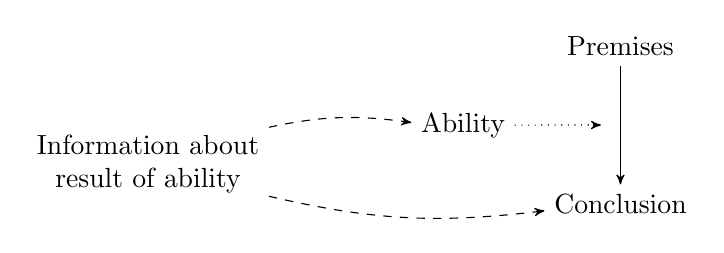
\begin{tikzpicture}[->,>=stealth',node distance=0cm, every text node part/.style={align=center}]

  \node (1) [] {Information about \\ result of ability};
  \node (2) [right of=1, xshift=4cm, yshift=.5cm] {Ability};
  \node (3) [above of=2, yshift=1cm, xshift=2cm] {Premises};
  \node (4) [below of=2, yshift=-1cm, xshift=2cm] {Conclusion};

  \draw [dashed, ->] (1) to [bend right=10] (4);
  \draw [dashed, ->] (1) to [bend left=10] (2);
  \draw [->] (3) to node[left] (mid) {} (4);
  \draw [dotted, ->] (2) to (mid);
\end{tikzpicture}
\caption{Sketch of support.
  Continuous arrow is direct.
  Dashed is indirect from information.
  Dotted is indirect from agent.}
\label{fig:dynamics}
\end{figure}

\begin{note}[Quick parallel]
  \(\vdash p \rightarrow q\).
  Though something more involved.
  And this goes to \(p \vdash q\).
  This isn't quite the full story, as there is also the interpretation of \(p, q\), etc.
  And \(p \vdash q\) might not capture the way in which \(q\) follows from \(p\) when interpreted.
\end{note}


\begin{note}[Variation on a familiar problem]
  This is a twist on a familiar problem.
  Lots of ways to explain why an agent performed an action.
  Here, the agent is picking one of those ways.

  Problem is to identify the actual from the potential reasons.
  Here, our agent has a guarantee of potential reasons, and acts on the basis of those.
  If the agent could, then the agent is.

  With sufficient information about potential reasons, may an agent from appealing to those reasons when performing an action?

  justification footnote\nolinebreak
  \footnote{
    A different way to motivate the idea is through propositional and doxastic justification.
    As, the agent has a guarantee both that they are propositionally justified, and that they have the ability to be doxastically justified.
  }
\end{note}


\begin{note}[License]

  \begin{quote}
    A license allows an agent to support some result with reasons (or reasoning) that obtain(s).
  \end{quote}
  License is that those reasons do obtain.
  License includes information about what the result is, but does not include complete information about how the result is obtain from the reasons (or reasoning) that are licensed.
  In the chess example, there is partial information, but there may also be cases with no information.

  Need assurance that license is good.
  Hence, the role of the agent's ability.
  I assume that the agent's ability is involved.
  This may be redundant.
  Difficult.
  Distinction between internal and external reasons.
  Ability makes this a little fuzzy, and this is why there is appeal.
  Supports the idea that these would function as internal reasons.
  If the agent does not have the ability, then the same may still hold.
  For example, passing reasons between agents.
  Agent A grants agent B license to appeal to the reasons that agent A has in order to agent B to obtain a result.
  Etc.
\end{note}

\begin{note}
Agent reasons, generates considerations and so on.
The agent is able to witness such reasoning.
See how the conclusion depends on the premises.
But the conclusion does not depend on the agent's ability to reason.
The conclusion cannot be false without the agent losing the ability to reason.
Right, because the reasoning is (in part) what makes it true that the agent has the ability.
Without the reasoning, there is no ability.
The agent's ability does not, and can not, be substituted for such reasoning.
\end{note}

\begin{note}[Async]
  Somewhere in here mention the idea of asynchronous reasoning.
  The reasoning doesn't (or reasons don't) necessarily stay potential.

  This ties to bounded agency, and part of the `why' question.
\end{note}

\begin{note}[Why]
  First question is why?
  In the chess example, the agent is only able to conclude that a winning strategy exists.
  On the one hand, it must be true.
  On the other hand, there is reasoning that demonstrates a winning strategy.
  Distinct, but the result is the same.

  This is reasons and chess.
  Not all reasons are interesting, so perhaps it's an effort to expect too much.

  Have already seen a potential difference.
  The role of the assertion, and what supports.

  Co-dependence, and idea that proposition that I have the ability does work.
  So, co-dependence observes that I can't really avoid making reference to the claim as a guarantee.

  This isn't so simple though.
  If I did the first instance of reasoning, then I've avoided appeal to my ability.
  Hence, if I go about finding a strategy and start to doubt my ability, then I only doubt that a strategy exists because this impact the general truth of what you say.
  However, on the second instance of reasoning, then I've appealed to my ability, and I get a straightforward bit of reasoning to the non-existence of a strategy.

  So, there is a difference in dynamics, arguably.
  Difference between the reasons being inaccessible and the reasons not existing, (very) roughly.

  However, also want something positive\dots
  The difficulty is that the conclusion is not too interesting.
  So take \citeauthor{Emms:2000aa}'s original puzzle.
  Have the ability to show that there is checkmate for Black in four moves.
  If this is the case, then can tell this to White, and White may resign.

  This may be considered cheating.
  It is certainly cheating if the agent playing Black relies on information provided by a third party.
  It would not be cheating if the agent playing Black found a strategy.

  Some cases finding the strategy is of interest.
  Still, if the agent has the ability, and neither agent is particularly interested in the end game --- perhaps they want to practice the mid game --- then there's little point in playing through.
  So, assume that providing a strategy is of little interest.

  Suppose Black does the second kind of reasoning.
  Does Black cheat (on the particular understanding of cheating given)?
  The support offered is the reasoning that the agent is able to do, and this is the agent's reasoning.
  If White were to challenge, expect Black to provide the strategy --- not insist that such a strategy must exist.
  That Black was informed of their ability simply \emph{licensed} Black to appeal to those reasons.

  Black did not obtain a victory by appealing to information that they could not support.

  Well, truth is difficult.

  Second example, Morse and Lewis.

  Structurally the same.
  Issue is whether the reasons why an agent holds a proposition to be true matter if these do not affect whether or not the proposition is true.
\end{note}



\hozlinedash



\begin{note}[Upshot/Idea of a generator]
  The upshot is that the agent is confident that they can generate an explanation.
  Therefore, the adoption of the conclusion is backed by these additional considerations.

  Really need the shopping example (or something similar) to make this point particularly interesting.

  \hozlinedash

  The ability to reason guarantees that there is a strategy, and that you can demonstrate what that strategy is.
  Term this a \emph{generator}, as the execution of the ability generates a demonstration.

  Generators are what this paper is (directly) about.
  Your ability to reason from the rules of chess and the game state to a strategy for Black is a particular instance of a generator, and serves as the template for an abstract characterisation:
  A generator is something that, if witnessed, provides reasoning in support of a conclusion.

  This paper is (indirectly) about how reasoning supports a conclusion.
\end{note}

\hozlinedash

\paragraph{ }
\begin{note}
  Space for a technical summary \& overview here.

  To add is an enumerated outline of the agent's reasoning.
\end{note}

{
  \begin{note}[Important]
    For, it is open to think of the possible reasoning simply as an elaboration of why the designated value is preserved.
    If so, then it's hard to see a difference between the two instances of reasoning, as both succeed at establishing that the conclusion must be true.

    In a way, the preservation of truth is derivative of the reasoning that the agent is able to do, as the contents of the propositions are, in a sense, interpreted.
  \end{note}

  But why does this matter?
  Often substitute reasoning by the flow of a designated value for interpretation.
  For example, one would expect that various scientific models have this property, as the mathematics used to capture the phenomena entails certain other things, and this may all be fine without getting at whatever it is that the mathematics is capturing.
}

Adopting a broader perspective, reasoning is a activity in which a conclusion is obtained from premises.
Conclusion of interest is hold it to be true that White cannot prevent Black from occupying c4 on their second move.
The premises concern the rules of chess, the game state, and perhaps claim~\ref{chess:claim:1}.

Able to do the reasoning.
Label these \emph{directly supporting} premises.

However, unless an agent has reasoned from the premises to the conclusion, the agent requires additional information to be confident that they are able to reason from the directly supporting premises to the conclusion.

Yet, the additional information is not required as a premise in the reasoning the agent is able to do.
In this way, the additional information is not a directly supporting premise.
For, any additional premise is required only because the agent has not (yet) done the reasoning.
Can be sure that it is redundant because these simply recognise what the agent's ability is (so this is potentially a restriction on additional inputs being considered.)

So, in the reasoning you do, there is a distinction between the premises which directly support the conclusion and those premises which inform an agent that the conclusion follows from those directly supporting premises.




So, get a distinction between directly supporting premises and indirectly supporting premises for the conclusion of reasoning that the agent does in order to establish the conclusion.



With a distinction between directly and indirectly supporting premises comes the opportunity to distinguish the directly supporting premises.
Directly supporting premises are those which {\color{red} guarantee} the conclusion (from the agent's point of view, at least).
In this sense, the agent's ability and the directly supporting premises are those premises which explain \emph{why} the agent holds the conclusion.
However, without the indirectly supporting premises the agent's ability and the directly supporting premises do not explain \emph{how} the agent came to hold the conclusion.

% \emph{Still}, the directly supporting premises do not justify the agent.
% Instead, the directly supporting premises guarantee that the agent can generate `direct' support for the conclusion.

So, agent's ability and the directly supporting premises are those premises which explain \emph{why} the agent holds the conclusion.
There is a difference between reasoning from the premises of the rules of chess and the game state to the proposition.
However, distinguish (at least) two kinds of explanation.

Ability explains because factive inference.
Hence, conclusion must be true.
However, this explanation for why the conclusion must be true if the premises are true does not explain why the conclusion follows from the premises.
The reasoning demonstrates a strategy.
Move from some information to some other information.
Explanation of why the preservation of truth occurs.
The ability only guarantees that a strategy can be found.
Ability only guarantees that some information can be obtained from other information.
Explanation of why one can be confident that preservation of truth occurs.

\hozlinedash

An alternative thesis may assume that the agent is justified, and then demonstrate the way in which the reasoning outlined justifies the agent holding the conclusion.
Perhaps this is correct.
I have no provided an account of justification, and it may be that the explanation that the agent cites is also justification.


And, as the agent is confident that they can witness such reasoning, this provides the agent with a guarantee that the conclusion holds.

The agent has the ability to reason from the premises to the conclusion, but the conclusion follows from the premises independently of whether or not the agent has the ability.
In this sense, the fact that the agent has the ability is independent of whether or not the conclusion follows from the premises.

propositional/doxastic\nolinebreak
\footnote{
  Frame this in terms of propositional and doxastic justification.
  Here, the agent has a guarantee that they have proposition justification, and that they can generate doxastic justification.
  However, the guarantee itself is not doxastic justification.
}


\begin{note}[Constructive]
  An important point here is that the agent's reasoning is non-constructive, in a sense.
  For, the agent has a guarantee that the conclusion is true, but the agent does not establish \emph{why} the conclusion is true.
  Hence, there are (at least) two `why' questions.
  \begin{itemize}
  \item Why the conclusion follows from the premises (and the agent's ability), and
  \item Why the agent holds the conclusion to be true.
  \end{itemize}
  If the agent were to do the reasoning, then these would both be answered.
  The explanation of why the agent holds the conclusion to be true (from the agent's point of view) is the same explanation as to why the conclusion follows from the premises.

  Something like, knights can move \dots, the knight can be captured only if \dots, the knight cannot be captured.
  White can only move to \dots, etc.\

  So, we can see that the agent has the ability to answer the first question --- why the conclusion follows from the premises.
  However, because the agent has not done the reasoning, this does not answer the second question.

  Still, the agent's ability guarantees that an answer to the first question may be generated by the agent.
  This is reminiscent of \citeauthor{Davidson:2001aa} \dots
\end{note}


\begin{note}[Davidson]
  \begin{quote}
    Because justifying and explaining an action so often go hand in hand, we frequently indicate the primary reason for an action by making a claim which, if true, would also verify, vindicate, or support the relevant belief or attitude of the agent.

    \vdots

    The justifying role of a reason, given this interpretation, depends upon the explanatory role\dots
    \nolinebreak
    \mbox{}\hfill(\cite[8]{Davidson:2001aa})
  \end{quote}

  If \citeauthor{Davidson:2001aa} is followed, then justification only if explanation, and explanation only if causation.
  So, justification only if causation.
  But this presents a problem.
  For, the agent's ability has not been witnessed, and therefore the justification that would be constructed cannot stand in any causal relation to the agent adopting an attitude toward the conclusion.

  The idea expressed above mirrors the interaction \citeauthor{Davidson:2001aa} points to.
  For \citeauthor{Davidson:2001aa}, justification indicates how to construct a primary reason which explains.
  In our case, primary reason indicates how to construct justification.

  So, this is a problem.
  {
    \color{red}
    Either the agent's ability does not do any justificatory work, or there is justification without causation.
    \emph{However}, this misses an alternative.
    The justification isn't the focus.
    It's the guarantee of justification.
  }
  The first option may be preferred.

  Have some reasoning, seems okay.
  Therefore, this provides justification.
  I struggle with this.
  The agent's reasoning obtains a guarantee of truth.
  However, this is `simply' \(\phi \rightarrow \psi\), without understanding why \(\phi \rightarrow \psi\).

  Contrast to a simple model of testimony.
  You have justification.
  Hence, the hearers justification goes by way of the speakers justification.

  The details of causation matter.
  However, abilities (or what would result from abilities) avoid some of the issues here.
  For, nothing is witnessed.

  It is somewhat interesting that \citeauthor{Davidson:2001aa} emphasises that one often doesn't have the primary reason, and instead provides information that is sufficient to generate the primary reason.

  So, the idea that an explanation can be generated is stressed by \citeauthor{Davidson:2001aa}.
  Difference is that \citeauthor{Davidson:2001aa} makes use of this idea when providing information about explanations.



  \begin{quote}
    Central to the relation between a reason and an action it explains is the idea that the agent performed the action \emph{because} he had the reason.
    Of course, we can include this idea too in justification; but then the notion of justification becomes as dark as the notion of reason until we can account for the force of that ‘because’\nolinebreak
    \mbox{}\hfill(\citeyear[9]{Davidson:2001aa})
  \end{quote}
\end{note}

\begin{note}[Generator]
  The core idea is that the agent's ability is something of a \emph{generator}.
  Where, a generator generates reasons.
  I am not claiming that ability statements are unique in this way, but they do have this feature, and therefore work as motivation.

  Now, the existence of the generator does some work in the causal explanation, so to speak.
  It is part of the reasoning that the agent does.
  The issue is about how it fits, with the idea being that one needs to turn it on (figuratively) to get the support that the agent cites, or the justification for the agent's action.
\end{note}


\begin{note}[Testimony comparison]
  Suppose you have my testimony that:
  \begin{itemize}
  \item If the rules of chess are in play and the board is arranged as in figure~\ref{fig:chess:move}, then While cannot prevent Black from occupying c3 on Black's second move.
  \end{itemize}

  This is slightly different to what is going on in the reasoning.
  Here, you do not have justification for the conditional, but you have justification for the claim being true.
  So, you can use the conditional in further reasoning.

  The present case is different.
  For, you are relying on the ability to generate justification.
  This conditional is not part of your reasoning, at least not initially.
  Rather, this conditional is obtained (if it is obtained) by noting that the conclusion must hold if you have the ability.
  So, here again the ability is doing the work.

  {
    \color{red}
    Footnote:
    This is not to take a stand on testimony.
    The reasons that justify in the case of testimony may be those of the speaker.
    However, if this is so, then there is still this distinction between \(\vdash \phi \rightarrow \psi\) and \(\phi \vdash \psi\).
    Hum, but then in this case, the existence of reasons does the appropriate work.
    Hence, there is a clear parallel.
    Still, in a sense these may be considered `witnessed', and my main concern is with the `un-witnessed' reasons by ability.
    Point being that if testimony, then it's not always going to be the case that the agent's ability is relevant.
    So, this marks a difference.
    Even if we think of ability as providing testimony, there's still something more, because testimony does not, in general, allow the agent to claim access to those reasons/that justification.
  }
\end{note}

\subsection{Examples}
\label{sec:examples}

\begin{note}[Difference between chess and shopping]
   The issue is that the agent hasn't worked through the reasoning --- \emph{not} that the agent is unaware of the reasoning required.
  This is an important distinction between the chess scenario and the shopping scenario.
\end{note}

\subsection{Ability}
\label{sec:ability}

\begin{note}[Issues with simply talking about ability --- verifying vs.\ solving]
  Similar to calculators.
  \(7^{3} = 343\), but I do not consider the result of computer program a reason to hold that \(7^{3} = 343\).
  The program informed me that, given my understanding of arithmetic, I may hold that \(7^{3} = 343\).

  Compare to:
  \(\lim_{n \to \infty}\left(1 + \frac{1}{n} \right)^{n} = e\)
  This goes beyond my ability.
  If the computer program provides an explanation of how the result was derived, I may study the steps and identify ways to develop the ability, e.g.\ by developing an understanding of l'H\^{o}pital's rule.

  While there is an intuitive distinction between the ability to show that \(7^{3} = 343\) and the ability to show that \(\lim_{n \to \infty}\left(1 + \frac{1}{n} \right)^{n} = e\), there are intermediate cases which put pressure on what is meant by the ability to reason from \(\Sigma\) to \(\phi\).
  For example, I doubt I have the ability to solve \(\sqrt[5]{59049}\) without some assistance, but I do have the ability to show that \(9^{5} = 59049\), and hence the ability to verify that \(\sqrt[5]{59049} = 9\).

  I consider both the ability to solve and the ability as instances of ability to reason, but keeping track of the differences is not too important.
  Therefore, to keep things simple I take talk of the ability to reason to align with the ability to solve.
\end{note}


\section{Explanation}
\label{sec:explanation-1}

The broad objection brewing here is that the agent representing themselves the structure of their reasons in a particular way doesn't necessarily demonstrate anything of interest.

\begin{itemize}
\item Some sort of error theory?
\item This is different from claiming that the agent is \emph{irrational}.
  \begin{itemize}
  \item This is an issue that I want to set aside for now.
  \item I don't think that licensing necessarily involves irrationality --- some instances may be rational, other irrational.
  \item The issue depends on broader perspectives.
  \item For example, with the shopping scenario.
    If the agent buys the star fruit and this results in benefit to them, then it may be rational.
    If correctly responding to reasons, then arguably irrational, as the agent does not respond.
  \item Issue, really, is whether this \emph{actually} happens.
  \end{itemize}
\item Perhaps: Back to the remarks of \citeauthor{Davidson:2001aa} about explanation.
\end{itemize}

\subsection{Preservation of a designated value}
\label{sec:pres-design-value}

{
  \color{red}
  I think this is where the main work is.
  Need to show that reasoning in the relevant cases doesn't reduce to the preservation of a designated value.
}

\begin{note}[Two types of ability]
  In the cases of interest --- ability to reason --- the ability does not \emph{make} the conclusion true.
  The conclusion is available to the agent because it holds independently of the agent's ability.
  Contrast to other instances of ability, such as running a 5K, where the executing the ability would make the relevant proposition true, but without the execution there is no way to obtain the truth of the proposition.

  Hence, in the case of ability to reason, there must be something other than the agent's reasoning which is securing the truth of the (relevant) proposition.
\end{note}



\begin{itemize}
\item \emph{Reasoning just is the preservation of a designated value}.
\item The designated value is true, utility, etc.
\item If this is so, then there's nothing more.
\item This is a strong argument, as nothing (of interest) can be gained by generating the additional reasoning.
\end{itemize}

\begin{itemize}
\item \emph{This is may be quite standard.}
\item Think about practical reasoning.
\item Means-end, in particular, and how necessity is invoked.
\item The supermarket is useful here, as on one reading, I have shown that I must buy the star fruit, but on another reading I have demonstrated why buying the starfruit would do something for me.
\end{itemize}

\subsection{Mental state}
\label{sec:mental-state}

{
  \color{red}
  The main idea, really, is that I end up `wrapping' many principles in a conditional of the form:
  \begin{quote}
    If full explanation then (\emph{Principle})
  \end{quote}
  So, if you're into a particular principle, you get to keep this principle, so long as you don't also hold that the principle is sufficient for a full explanation.

  It seems, perhaps, the most will not hold the converse.
  For, cases of deviance.
  Deviance also helps to demonstrate the general use of a wrapper --- restrict to particular cases.
  However, one may wish to drop the `full' from the wrapper, and claim the principle holds whether an explanation is available.
}

I think, potentially, that a number of these objections can be grouped under the idea of a reason or reasoning being a mental state.

\subsection{Actual reasoning}
\label{sec:actual-reasoning}

\begin{note}[Ability]
  Distinction between:
  \begin{itemize}
  \item The agent's ability.
  \item The property of the agent that they have the ability.
  \end{itemize}
  This is an important distinction.
  The agent's ability is not, in general, a property of the agent.
  Ability involves actions/events.
  But these can be referenced by a predicate.

  So, the structure between the premises and conclusion is done by the ability, not the property.

  This is `the factive inference'.

  Still, one may distinguish between the fact and the considerations which result from a factive inference.
  This is fair.
  And, this allows us to some flexibility.
  However, there is a difference between the fact and the considerations.
  For, the considerations have partial information, while the fact \emph{is} the information (speaking loosely).
  So, it does not seem possible to completely move away from the agent's ability.
\end{note}

\begin{itemize}
\item Objection is that the agent's confidence in their ability is `enough' of an explanation.
\item Reminiscent of an idea from Williamson, and recently put to use by \citeauthor{Lord:2018aa} (and maybe \citeauthor{Kiesewetter:2017aa}).
\item Here, the factive entailment is enough for an explanation, very roughly.
\item In this way, one can explain by appearances, and this does enough.
\item However, the issue is with the \emph{kind} of explanation that is obtained.
\item The factive inference gets a truth-truth/non-constructive explanation.
\item The conclusion must be true, but this does not constructively explain why the conclusion is true.
\item So, this doesn't really do anything, and the same issue arises for this kind of explanation.
\item The inference is truth-truth, with the assumption of something else doing the work.
\end{itemize}

\begin{note}[The Williamson idea]
The Williamson idea is that it's reasonable to hold that appearance is factive.
Hence, \citeauthor[Ch.\ 7]{Lord:2018aa} and \citeauthor{Kiesewetter:2017aa} are able to argue that appearances provide reasons.
Not necessarily the same (kind of) reasons, but sufficient reasons.

(
As an aside, this is somewhat interesting because it provides an account of why appearances are reason-giving.
One could argue that this is independently true, but the interesting point is that objective reasons are non-redundant even if they are reason giving.
For, if there were no objective reasons then there would not be an entailment from appearance to reason.
)

The strategy doesn't apply to the cases that I am interested in.
For, this would require me that the agent's confidence in their ability provides a reason.
However, the natural understanding of the scenarios is that the agent relies on their ability to guarantee the existence of a reason, rather than the ability \emph{itself} being a reason.
\end{note}

\subsection{Causation}
\label{sec:causation}

The core idea here is that causation is only going to work if one thinks that the agent's reasoning provides a `complete' explanation.
I deny that the agent's reasoning provides a complete explanation --- the point of licensing is to secure a `complete' explanation without doing the reasoning.

Basically, the agent's reasoning needs to be part of the causal chain.

\subsection{Supervenience}
\label{sec:supervenience}

The idea is that supervenience is stronger than appealing to causation, because we have an argument for why the \emph{content} is not part of the explanation when appealing to supervenience (or the dependency strengthened version of supervenience).

I can't simply argue that there is more to the explanation, because if supervenience holds then there cannot be anything else.

\begin{note}[Structure]
  Overview of section:
  \begin{itemize}
  \item Supervene on internal mental states.
  \item This is a problem, as the agent's potential reasoning is not an internal mental state, seems one can vary ability without changing anything --- certainly true in general cases of ability.
  \item Whether this holds for reasoning in particular is unclear.
  \item Note, however, two kinds of supervenience.
    \begin{itemize}
    \item Reasons,
    \item Rationality
    \end{itemize}
  \item Interested in supervenience of reasons.
  \item The idea is that this rules out the agent's potential reasoning as being something that explains.
  \item It cannot stand in the role of a reason because the potential reasoning does not supervene.
  \item Plausible that ability supervenes, if supervenience is characterised broadly, which it may need to be.
  \item Arguably, this does not address the motivating intuition.
  \item As an aside --- in principle, supervenience is compatible with externalism about mental content, and one may argue that the licensing pulls in the reasoning in this way.
    \begin{itemize}
    \item Still, ability can vary without confidence in ability varying --- this subdivides the agent's mental states, but holds on to the same intuition.
      For, the agent's reasoning would go through without this --- the key is that supervenience establishes a kind of dependency relation, and the idea is that anything outside of this dependency relation is not required for an explanation.
    \item This entails supervenience, but is a little stronger.
    \item Supervenience is a particular kind of dependency relation, no?
    \item If one took up the aside, then we find that the external content would be redundant, only some of the state matters.
    \end{itemize}
  \item So, this provides an argument for the idea that the agent's potential reasoning being redundant.
  \item The argument isn't perfect.
    For, there are cases where it doesn't seem as though one can strip away redundancy --- e.g.\ \(p, p \rightarrow q, q \rightarrow r\) hence \(p \rightarrow r\) by conditional proof and hence \(r\) versus detaching the way through --- as one has already done this in the conditional proof so it seems redundant.
    Still, I take the broad strokes to be sufficiently clear.
  \item A consequence of this is that by using something in reasoning it becomes a reason.
  \item The agent is going to get to the conclusion whether or not they have the ability.
  \item Evil demon cases.
    \begin{itemize}
    \item We see that the agent only needs the relevant premises.
    \item But, may not need the demon.
    \item Example where premises of reasoning may no longer hold.
    \item May think that this is the same as, for example, memory, where the thing remember may no longer hold.
      However, here we often take memory itself to be the source, not the thing remembered.
      Licensing suggest this need not be the case, but the problem remains.
    \end{itemize}
  \item So, the agent's ability is not a premise, only the agent's confidence that they have the ability is a premise.
  \end{itemize}
\end{note}

\begin{note}[Main points]
  Supervenience is an interesting take.
  Need to show that the potential reasons do not supervene.
  This is not obvious.

  The simplest way to object to this is to note that what the agent has an ability to do varies given other things.
  Some easy examples of this, such as the arrangement of tennis players in a tournament.
  The order of play may determine whether or not the agent has the ability to reach the grand final.
  As, particular adversary, but they're weak to another player, that the agent is strong against.
  Hence, the draw may work out in the agent's favour.

  Does the same phenomena arise with reasoning?

  There's also the issue of factivity, which \citeauthor{Singh:2019aa} notes.

  The way I \emph{want} to object to this is to claim that the agent does not, in the appropriate sense, have a motivating reason.
  The agent \emph{needs} the factivity to get the motivation.
  Hence, without this there is no reason to speak of.
  There's nothing to `get' from the agent's motivating reason.
  This restricts the scope of supervenience, in a sense.
  Not all reasons that motivate explain, or not all reasoning explains.
  (Not: not all reasons are motivating reasons --- not all reasoning is motivates.)
  Some ideas of \citeauthor{Lord:2018aa} seem to apply here --- some of our judgements about rationality apply, but not all.

  The above restricts the application of supervenience.
  An alternative is to argue that ability to reason does supervene on the mental.
  Hence, superveniece does not fail.
\end{note}

\begin{note}[Two superveniece claims?]
  Is there a distinction between the claim that reasons supervene and the claim that rationality supervenes?
  Possible, if rationality is insensitive to whether or not something is genuinely a reason.

  \begin{itemize}
  \item Rationality involves responding to reasons, etc.\
  \item Rationality is about structure, and whether or not structure is supported depends on ability.
  \end{itemize}

  The difference really does seem important.
  For, there are factive inferences all over the place, but if we restrict attention to the reasoning involved, then nothing goes beyond this.
  By analogy, it's the difference between validity and soundness.
  This is kind of what \citeauthor{Lord:2018aa} gets at with the idea of comparative rationality.

  So, the issue here is whether the agent has the same reasons in both cases.
\end{note}


\textcite{Singh:2019aa} has an extended discussion of supervenience.

\begin{quote}
  \textbf{Supervenience Constraint (SC)}: an agent’s motivating reasons supervene on the internal facts about her mental states.

  \vdots

  The internal facts about agents’ mental states are the facts about their non-factive mental states and the relations between them\nolinebreak
  \mbox{}\hfill\mbox{(\citeyear[6]{Singh:2019aa})}
\end{quote}

\citeauthor{Singh:2019aa} notes that this does not entail that nothing about an agent's motivating reasons can change without a correspond change in the agent's mental states.
For, it may be the case that a motivating reason switches between \emph{also} being a normative reason, depending on what the facts of the situation are.

{
  \color{red}
  There's also \citeauthor{Broome:2013aa}'s claim that rationality supervenes on the mind (\citeyear[151, etc.]{Broome:2013aa}).
}

\begin{quote}
  One such starting point, which I hope is uncontroversial, is that an agent’s motivating reason must play a motivational role (broadly understood) in her psychology.
  If it did not play this role in her psychology (that of motivating her, in a broad sense) it would not be her motivating reason.
  Thus, whatever a motivating reason is, it must be something that can play this psychological role.\nolinebreak
  \mbox{}\hfill\mbox{(\citeyear[4]{Singh:2019aa})}
\end{quote}

\begin{note}[Compatibility]
  First point is compatibility.
  Agent's ability to reason, perhaps this supervenes.
  Plausible, but this doesn't get to the real objection here.
  Ability may supervene, but agent's confidence may not.
  And this is where the problem starts.
  For, even if the ability supervenes, it's the confidence that the agent has the ability that does the work.
  And \emph{this confidence} does not supervene on the ability.
  The reasoning that the agent does is the same in both cases, even as we move around whether or not the agent has the ability.
\end{note}

\begin{note}[Motviation for supervenience/evil demons]
  The standard motivation for supervenience seems to be evil demon type cases.
  Here, factivity fails, intuitions about reasons remains roughly the same.
  Hence, factivity is not a principal component of the analysis, at least.

  \citeauthor{Singh:2019aa} has a nice line which links up to reasoning:
  \begin{quote}
    \dots since you reason exactly the same way to the exact same beliefs and actions, it remains the case that your motivating reasons are the same in both worlds.\nolinebreak
    \mbox{}\hfill\mbox{(\citeyear[5]{Singh:2019aa})}
  \end{quote}
  The intuition is that the reasoning would be the same.
  But this is tricky, and exactly where the distinction comes into effect.
  Agent's reasoning supervenes, but we need to stipulate that the agent's reasoning would be different if their reasons were different.
  If the demon cases hold, then whether or not a given mental state is factive is independent of whether or not an agent applies a factive inference to that mental state.
  Separate whether or not something is a reason from the use it has in the agent's reasoning.

  Then, need the entailment that something used as a reason is in fact a (motivating) reason.

  This generates a normative clash, as we get reasons from `nothing'.
  Agent need only treat something as a reason for it to be a reason.
  This is stronger than the claim that an agent may something act for reasons which are not normative, which leaves open the possibility of some constraint (e.g.\ guise of the good as endorsed by \citeauthor{Singh:2019aa}).
  \citeauthor{Schroeder:2007aa} takes this head on.

  Reasoning may be the same, with a difference in motivating reasons.
  Need a link between reasoning and something being a motivating reason for this to go through.

  Deny that this is the case.
  The agent's ability is such an example.
  This is not a motivating reason --- the unravelling of the ability is the motivating reason.

  Argue that this is a technicality.
  The intuition obtained from the evil demon cases applies to ability.
  Seems the agent is just as good in both cases.
  Don't even need the demon.

  But the evil demon situation is odd.
  In these cases there's something that the agent doesn't have access to, and we change this.
  By contrast, in the licensing cases, the agent's reasoning is purposefully incomplete.
  The agent's reasoning needs to be filled in.
  The result is the same, the agent obtains the conclusion, but the agent is sensitive to the risk.
  It's a basic trade-off.
\end{note}

\begin{note}[The evil demon]
  Some notes:
  \begin{itemize}
  \item It seems the evil demon only deals with the premises of reasoning.
  \item Typically factive premises, as this goes beyond the agent's reasoning.
  \item If the evil demon starts messing around with the reasoning, then it's really unclear what is going on.
  \item However, when dealing with licenses, we are not dealing with premises.
  \end{itemize}

  \begin{itemize}
  \item Comparison to an agent taking out a loan.
  \item Key component of this is the agent paying back the loan given agreed terms.
  \item Hard to determine whether or not the agent was okay when taking out the loan prior to repayment or default.
  \item There's uncertainty involved, and as the scenario develops and information is provided, this uncertainty is reduced.
  \item From the agent's perspective, given confidence, it's fine to take the loan.
  \item However, because of uncertainty, evaluation is tied to information, the loan is a bad idea if the agent has been fired while taking out the loan, and the agent is aware of this.
  \item Not changing the soundness of the premises here.
  \item Issue is that the evaluation is tied to information.
  \item So, we may get supervenience of our evaluation on available information.
  \item This is consistent with the evil demon cases, where the information available is the same --- factivity itself is not part of the information provided to the agent.
  \item All one needs in the factive inference.
  \end{itemize}
\end{note}

\subsection{Externalism}
\label{sec:externalism}

\begin{note}[Maybe?]
  Can I make use of a distinction between \emph{potential} reasoning and \emph{external} reasons?
\end{note}

\begin{note}[Supervenience]
  Perhaps restructure some of the supervenience observations here.
  I.e.\ because we're interested in reasoning ability, it seems this may be compatible with supervenience.
  For sure, the claim is restricted in this way.
  If agent appeals to explanations \emph{other} than their ability to reason, then it seems plausible that supervenience may fail.
  However, this is independent of the focus point, and may be taken up elsewhere.

  I mean, in short, if the intuition goes via twin duplicates, then it seems as though these should have the same reasoning ability.
\end{note}

\section{Loose ends}
\label{sec:loose-ends}

\subsection{Non-voluntarism}
\label{sec:non-voluntarism}

The main focus of the paper has been indirect access to reasons.

With non-voluntarism, the same ideas apply, but rule out certain conclusions.

It's the denial of an existential.

If the existential provides access and allows a conclusion to be adopted, and this holds in converse, then we've got a clear account of when an agent does not have the option of adopting a conclusion.

Hmm, there are two instances of this claim:
\begin{enumerate}
\item Adoption requires ability, hence if no ability then no option to adopt.
\item Ability along with exclusivity rules out certain options.
\end{enumerate}

\subsection{Weakness of will}
\label{sec:weakness-will}

Also could be framed as counterfactual ability.
Cases of rational impairment and so on.

In a sense, the issue here is the strength of the conclusion.
It seems the conclusions obtained while sober often extend and hold when intoxicated.

However, by contrast, conclusions obtained with full information may not.
E.g.\ \cite{Smith:2004aa} or the miners paradox.

This is something of a promissory note, then.

\section{Summary}
\label{sec:summary}

\newpage




\begin{note}[Main issue]
  A guarantee of an explanation may in turn be an explanation.
  (In a similar way to how evidence of evidence may be evidence.)
  However, that some thing may be an explanation does not establish that the thing is an explanation.

  In this way, the agent's ability is not a reason, in the standard sense of the term.
  For, the agent's ability is a matter of possible actions and events that, in general, go beyond the internal states of the agent.

  In short, the agent does not have an explanation for why they hold the attitude.
  However, the agent has a guarantee that there is an explanation.

  This may seem like misdirection.
  It is the property of the agent having the ability, or the inferences that the agent makes from their recognition that they have the property that does the work.

  Idea here is that the reasoning that the agent has done provides an explanation.

  However, this argument can be applied to all reasoning, so no facts are important.
  Hence, can improve on this with causal arguments.

  From one perspective, if the agent were to learn that they do not (in fact) have the ability, the agent would retain an explanation for why they came to hold the attitude.
  This is similar to how mistakes can explain, the fact can do some explanation, but it still seems as though the agent has an explanation if they were mistaken about a fact.
  Still, this does not work as an explanation from the point of view of the agent.
  Following Hieronymi \dots don't need facts.
  However, this seems to confuse two distinct things.
  On the one hand, there is the content of the mistake.
  And, on the other hand there is the mistake.
  Two different kinds of explanation, but the slip is easy.
  No longer have an explanation from the agent's point of view.
  Shift from the agent's point of view to what constituted the agent's point of view.

  \citeauthor{Hieronymi:2011aa}'s point is something like `the agent is the explanation'.
  {
    \color{red}
    Idea is that if we just look at the content, then we're missing part of the causal network.
    The explanation from the agent's point of view is not the `complete' explanation, because the agent themselves is part of this.
    Heck, this is complex.
  }

  Explanations have a causal trace, and if an ability has not been witnessed by some event, it cannot be the cause of anything.
  Hence, whatever would be from the agent witnessing their ability to reason cannot be the explanation for why the agent holds the attitude (without the agent witnessing the reasoning).

  Natural to expect that the agent's reasoning leaves the appropriate causal trace.
  So, it must be the case that the reasoning which the agent has done explains, from the agent's point of view.

  However, this goes too fast.

  Need the agent's reasoning.
  This point is made by \citeauthor[233]{Davidson:2001aa}, \citeauthor{Hieronymi:2018aa}, etc.
  And, once the agent's reasoning is in the picture, we're back to attempting to understand how the generator fits in with the agents reasoning, and hence the initial question; whether the agent needs to work through the reasons which settle.
\end{note}


\begin{note}[Ability and the environment]
  This is difficult.
  It may seem that in the case of reasoning, the agent's environment doesn't make a difference.
  Any ability can be traced to the reasoning that the agent is able to do, and the environment can only complicate by preventing the agent reasoning.
  For example, time or resource limitations.
  In the chess scenario, there isn't much interaction, but I doubt that in general an agent can be isolated from their environment in an interesting way.
  For, gaining information.
  Agent's ability to reason may be tied to information being within their epistemic reach, so to speak.
  Detective with a notebook.
  Detective has the ability to reason, but this is tied to the agent recalling information from their notebook.

  This is not to deny that a distinction can be drawn.
  May say that an agent has an ability given the information that they have, has an ability given the information that is within their epistemic reach, has an ability given the information they ought to have, and so on.
\end{note}


\newpage
\begin{note}[Does basis vs.\ reasons help with supervenience]
  Does basis vs.\ reasons help with supervenience?

  More verbosely:
  There are additional, specific, reasons that demonstrate the possibility of a particular move.
  However, this is the result of some reasoning rather than an input to some reasoning.

  The issue is whether the agent is appealing to the \emph{existence of reasons} or the \emph{possibility of reasoning}.
  These are, arguably, two different things.
  I think the supermarket case incorporates both, but (at least in the basic cases) it is the possibility of reasoning (which would generate reasons) that is of interest.

  {
    \color{red}
    This doesn't seem right.
    It's not clear how to get reasons to do work without reasoning (at least given my focus), hence there's no appeal to the existence of reasons without appeal to potential reasoning.

    {
      \color{blue}
      This note should be in the introduction where I lay out my use of reasons.
    }
  }
\end{note}


\hozlinedash


\newpage

\section{??}

\subsubsection{Objection}


\section{Interest}
\label{sec:interest}

The main upshot is in cases where the set up is not so simple.
The claim in the chess scenario (and other scenarios) ensured that reasoning went via ability.
Still, similar reasoning may apply to more standard cases of receiving information.
Need:
\begin{enumerate}
\item Information that some conclusion follows from some reasoning.
\item Confidence that the agent is able to perform the reasoning.
\end{enumerate}
If both these conditions obtain, then the agent may be confident that they are able to generate an {\color{red} relevant kind of} explanation.

\section{Supervenience}
\label{sec:supervenience-1}

\begin{note}
  The broad issue here is that one doesn't want to tie rationality to `objective' reasons.
  For, in many cases an agent may be unaware of what objective reasons there are, and yet this does not seem to entail that the agent is not rational.
  So, e.g.\ \citeauthor{Lord:2018aa} and \citeauthor{Kiesewetter:2017aa} restrict which objective reasons are of interest.
  These are those reasons which are recognised.

  So, subjectivism is a worry here.
  For, it's now the case that the agent may not be able to determine what they ought to do.
  Or something, though this objection is odd.

  Well, a better way to put the issue here is that we're interested in reasons, and how these relate to the agent doing stuff.
  Therefore, there's something normative going on.
  Yet, if we're interested in objective reasons, then it is unclear how one is going to obtain any applicable normative concept, as the agent doesn't have the information required to determine the normative state that obtains.
  Therefore, there must be some derived subjective normative state.
  But, then this simply appears to be the standard subjective normative state.
\end{note}


\begin{note}
  The link to rationality is not so smooth.
  For, one may argue that rationality should be divorced from responding to reasons.
  Instead, it is premised on agent's attitude toward what reasons they have.
  If this is the case, then the two positions are compatible.
  However, whether an agent is rational or not will then not depend on what reasons the agent has.
  For example, \citeauthor{Broome:2013aa}'s account of enkrasia is premised on the agent's belief about what reasons they have.
\end{note}

To demonstrate the problem, consider two contrasting situations.
In one situation the agent has the ability to respond to some reason, and in the other the agent does not.
The difference is generated by the presence or absence of some information within the agent's grasp.
For example, whether or not there is supporting evidence.

A cleaner example with respect to my view is that an agent is able to form a dependency relation of reasons that they do not have direct access to.
And, in these cases the agent is rational if those (independent) reasons exist, and is not rational otherwise.
However, if this is the case then the agent's rationality does not supervene on their mind, for the existence of the reasons in (by definition) independent of the agent's mind.
Hence, the supervenience claim must be denied.


\subsection{Difference in the kind of case}
\label{sec:difference-kind-case}

There is a difference in the kind of case.
For, in the demon style cases it is not particularly clear what it is that the agent could do differently.
This is something like an ought implies can principle.
The idea, roughly, would seem to be that if the expected reasons do not obtain in the bad case, then some other reasons do obtain.
Yet, as the agent is in the bad case, then agent is unable to access whatever it is those reasons promote.
Hence, as the agent is unable to respond to those reasons, then those reasons can not be normative.
This \dots is interesting.
One then also needs the claim that ether set of reasons is normative, and then the conclusion follows by disjunctive elimination.
I.e.\ something determines what the agent is to do.
I mean, the easy version of this is performing the same argument for anything that the agent does not recognise.
One can always construct a different case, and therefore these can't do the work.

\begin{itemize}
\item The agent is able to respond to reasons.
\item For any reason not recognised by the agent, it is possible for the reason to not obtain and the agent to remain the same.
\item If the reason does not obtain then it is not possible for the agent to respond to the reason.
\item It is not possible to determine whether or not the reasons not recognised obtain.
\item So, it is not possible for any reason not recognised to be normative.
\end{itemize}

It's something more like transparency.

\begin{itemize}
\item Reason only if the agent can determine whether or not it obtains.
\item Agent cannot determine whether or not factivity obtains.
\item Factivity cannot be a reason.
\end{itemize}

This sort of argument generalises to ability, in a sense.

This strays a little from the core intuition, which was that the relevant issues in the demon case were outside the control of the agent, whereas in the ability case the agent has the option of relying on their ability.

Hence, there is an argument that the idea of motivating internalism by demon cases isn't so clear.
For one may think that demon cases remain an issue on this picture.
For, there's nothing about the claim that ability can matter which requires a difference in rationality between the demon cases.

This is probably a useful observation to make.
If the motivation for internalism comes from demon cases, then it's not a good argument for internalism.
For, this is a non-internalist position which does not require there to be a difference in the demon cases.

On the other hand, one has a way to generate demon-like cases, so an argument agains texternalism will go through.
However, this argument cannot be premised on intuitions regarding demon cases.
That is the single upshot of this observation.

Yet, it seems quite weak.
For, the intuition is that two situations that are indistinguishable from the point of view of the agent are indistinguishable from the perspective of rationality.
And, this is going to occur in cases of ability.
If the demon cases are illustrating this distinction, then there's nothing to really be said.

Right, it's hard to see how this can really be useful.
For, the issue is whether all reasons are represented.
I can agree that all represented reasons are internal in the relevant sense.
So, I can agree that the demon case doesn't make a difference to represented reasons.
In this sense the `looking the same' is the relevant intuition.
Where I depart is in whether representation is all that matters.

So, the only thing of use is the idea that it \emph{might} be the case that one has a representationalist presupposition in the demon cases.
This is how I can claim compatibility with the demon cases, yet still push for something of an externalist flavour.

\hozlinedash


\section*{Outline}
\label{sec:outline}


\begin{itemize}
\item As an attitude, there are (at least) two questions of interest
  \begin{enumerate}
  \item When is the agent permitted to hold this attitude
  \item What is permitted given on this attitude.
  \end{enumerate}
\item The second question is difficult.
  This can be seen by thinking about belief.
  Here, the Lewis example is useful.
  Lewis may have the belief that agent is guilty, have the evidence and so on.
  However, whether this allows Lewis to make an arrest is not clear.
  So, shouldn't expect anticipation to be any simpler.
\item The first question is also difficult.
  Goal here is to provide necessary and sufficient conditions.
  Ideally we would have something extensionally equivalent.
  Ability, and how this is understood.
  Looking for something explanatory.
  Trade off between complexity and understanding.
  So, look to squeeze.
  Get a necessary and a sufficient condition, separate.
  Also a flexible tool.
\item So at the end of the paper I will have explained this kind of attitude, and outlined a key part of understanding the permissibility of the attitude.
\item Big thing is ability, and async.
\end{itemize}

\begin{itemize}
\item Understanding of support gives rise to phenomena.
\item Can understand how this can occur, even if there's no simple expression.
\item Explain how an essential part works, and a couple of simple results.
\item Upshot is some progress on ability and rationality.
\end{itemize}

{
  \color{red}
  Have the basic phenomena.
  Anticipation and ability, etc.
  Interest is in interaction.
  Conditionals of the form:
  \begin{itemize}
  \item Ability -> Permitted to anticipate
  \item Permitted to anticipate -> Ability
  \end{itemize}
  Necessary and sufficient conditions.

  These are, roughly, `reason why' conditionals.
  The ability is there to explain why the agent is permitted to anticipate something.
  However, partial explanations.

  This is due to there being various things to say about ability.
  The main problem here is that ability is a modal, so it's instances are going to depend on how the modal is understood.
  Unless the structural features do enough, then we need \emph{at least} need to supplement the account with information about the relevant alternatives.
  Further, it's not clear that this could provide a full explanation.
  Non0deal agents, and something tied so strongly to action.
  Pragmatic encroachment, etc.\ in knowledge, similar worries here.


  {
    \color{blue}
    One way of understanding things is that I am informed that I have propositional support (abstracting from evidential justification), and I am informed that I can also provide doxastic support.

    The main idea is that the agent is okay to anticipate because this is a truth oriented attitude.
    And, here the ability is important, because the availability of the truth of \(\phi\) holding on the basis of \(\Sigma\) is given by the agent's ability.

    If agent simply holds that \(\phi\) on the basis of \(\Sigma\), then the agent is not responding to reasons, etc.\
    Assume that responding to reasons is important.
    Instead, something like a safety condition.
    It is unlikely that the relevant reasons do not hold.
    So, the agent is responding in accordance with reasons, roughly.
  }

  {
    \color{red}
    So, the problem is arguing for the conditionals.
    What I want is an assumption that I can make use of.
    This is an assumption about permissible action.

    Reasons.
    Some accessible, other inaccessible.
    Recognised and unrecognised.
    Assumption is that an action is permissible if it is supported by the available reasons.
    Different from being supported by recognised reasons.

    Well, the main issue is with the attitude.
    So I'm wondering when it's okay to base my attitude toward \(\phi\) on \(\Sigma\), without having demonstrated that \(\phi\) follows from \(\Sigma\).

    So, I'm \emph{not} making a general claim about rationality.
    Rather, I'm interested in a fairly straightforward attitude, that is of interest for a number of reasons.
    The attitude is, roughly, about relations between mental states.
    Holding \(\phi\) on the basis of \(\Sigma\) (without having demonstrated).
    How the attitude is put to use is something else (can see in the Lewis scenario that one can toy with factors independent of the attitude to change whether or not it seems rational).
    First step is figuring out the attitude.
    So, looking at ability to reason.

    The argument is that this is an attitude of interest, and that there are these links to ability.
    This doesn't tell us that the agent is going to be able to do anything with the attitude.
    So, then, attitude with conjecture that it is rational for this attitude to be the basis of action in certain cases.
    Perhaps this is only due to the limited resources of the agent.
    Or perhaps the fact that an ideal agent will always have the results clouds more general observation.
  }
}


\begin{itemize}
\item Includes a fairly straightforward account of non-voluntarism, if a link between anticipation and belief is assumed.
\end{itemize}


\begin{itemize}
\item There are ways to complicate the basic puzzle.
\item The hypothesis here is that these are explained by the link between anticipation and action.
\item I assume a simple picture, where the agent is permitted to act on an anticipated proposition, but this isn't always going to be the case.
\item When this fails, it is due to limitations placed on what an agent can do with an anticipated proposition, rather than limitations on anticipation.
\end{itemize}



\newpage


\section{Literature}
\label{sec:literature}

\begin{itemize}
\item \textcite{Worsnip:2018aa}
\end{itemize}

The type of scenario I have outlined can be seen as a simple variation on a type of scenario consider by \textcite{Worsnip:2018aa} (among others).

The main difference is that in the case of \citeauthor{Worsnip:2018aa} there is testimony that \emph{indirectly} `destroys' the possibility of a structural relation.
Whereas in these kinds of cases there is testimony that \emph{indirectly} `creates' the possibility of a structural relation.

A cleaner parallel is with \cite{Christensen:2007aa} and the drug example.
This sort of issue is picked up on by \citeauthor{Neta:2019aa} (\citeyear[189]{Neta:2019aa}).

\begin{itemize}
\item In these scenarios an agent receives testimony that some reasons do not form a basis for holding a certain proposition to be true, but doesn't have access to `why'.
\item Contrast: testimony that some reasons do form a basis for holding a certain proposition to be true, but doesn't have access to `why'.
\end{itemize}

These arguments cause trouble for harmony between evidence and coherence.
This isn't something I'm going to explore.
However, if you are persuaded by coherence, then one way of understand the scenario I'm interested in is the recognition of coherence amongst attitudes.


\section{Objection}
\label{sec:objection}

It seems as though \citeauthor{Neta:2019aa}'s claim that reasons for which are always reasons why presents a difficulty for my account of what's going on.
For, it does not seem as though any of the indirect reasons can be reasons why.
A quick way to argue for this is to note that the reasons need not exist, and the story would continue in the same way, with the only difference being that my testimony is not truthful.

The core of the problem, then, is the claim that something can be a reason for which only if it can also be a reason why.
I sort of deny this.

The basic objection is that there is some rewriting.
Start with testimony, then rewrite so that testimony is avoided.

So, in a sense the reason that you came to hold the attitude is testimony.
Yet, this isn't the reason for which you now hold the attitude.

The issue here is whether some kind of causation is involved.
For, in the cases I consider it is for sure the case that no causation is involved.

A potential worry, then, is the divergence between causality and the agent's representation.
However, in these types of cases, the agent's representation is likely part of the causal explanation.
In that, it not only matters that the agent has an attitude, but it may also matter why the agent takes that attitude to be supported.

\citeauthor{Neta:2019aa}'s hybrid representational-dispositionalist view may be useful to consider here.

However, it's not super obvious that there is a conflict, in a sense.
Because, the `de dicto' existence is still represented.

Hm, the setup is:
\begin{itemize}
\item the agent wants star fruit
\end{itemize}
The question is:
\begin{itemize}
\item whether this is part of the explanation of why the agent purchases carambola.
\end{itemize}
The problem is:
\begin{itemize}
\item the agent does not represent wanting star fruit when purchasing carambola.
\end{itemize}

So, the argument against explanation is that the initial want is not needed when the agent performs the action.
It is clear that the \emph{specific} reason doesn't do any work (as this can be toggled without affecting anything else).
Therefore, one can look to the surrounding reasons.

So, either we have an instance of the relation that is not explanatory, or we don't have an instance of the relation.

{\color{red}
  The problem here isn't the possibility of the reason not existing, though this illustrate the worry.
  Rather, it is with the existence of the reason doing any explanatory work.
}
The problem is often raised with reasons first.
Roughly, the appearance of the reason is sufficient.

Still, this only goes so far.
For, it remains the case that the `supporting' reasons, so to speak, do the explanation.


\section{Why anticipation?}
\label{sec:why-anticipation}

\begin{itemize}
\item The phenomena is puzzling/interesting. (Whether possible\dots)
\item Make use of this kind of stuff
  \begin{itemize}
  \item Understanding how the structure differs from ideal agents, though shares certain features.
  \end{itemize}
  There may be other ways to understand what's going on here.
  However, this introduces complications.
  For, one needs to expand the basic understanding, and this may overgenerate.
  For example, with desire and testimony, it's kind of complex.
  If testimony alone, then other people, if only the agent, then what makes the agent's testimony unique?
  Avoid these problems by anticipating the relevant reasoning.

  Similarly, in cases of testimony there's a way to understand why the responsibility falls on the agent if they have the ability.
  \begin{scenario}
    Something of a test.
    I've got to come up with some answers, and then the file will tell me if I'm right.
    Not allowed to learn based on file.
    Have password.
    If the source is testimony, then I haven't learnt from the file.
    But, it seems that the file does the work.
    Confident that \(\phi\) on the basis of the file, because I can cut out the middleman.
    So the issue is whether this is permissible.
    Unclear.
    Difficulty is that there are typically many other factors.

    Another way to look at this is to ask whether I am the middleman can tell you.
    It's certainly not clear that learning by accident would be okay, though likewise it's not clear where the fault is.
    But this isn't unique to these scenarios.

    In footnote:
    Friends, playground has age limit, one is over, gate is open for repairs, owner only verifies one.
    Better with going into red barns, etc.
  \end{scenario}
\end{itemize}

{
  \color{red}
  Can argue that this reduces to testimony, of a kind.
  But there are cases where this would be unsatisfactory.
  \begin{itemize}
  \item Shopping list
  \item Morse and Lewis
  \end{itemize}
  Furthermore, if we are careful with constructing these scenarios, there are cases where testimony doesn't really work.
  \begin{itemize}
  \item Logic students.
  \item Wilson in a footnote.
  \end{itemize}
}


\newpage

\section*{Quotes}
\label{sec:quotes}

\begin{itemize}
\item If your IQ is higher than 85, you don’t need me to tell you that this line of reasoning depends on one very big and very false assumption\dots
  \begin{itemize}
  \item \url{http://racingweight.com/blog/tag/standard-american-diet/}
  \end{itemize}
\item You don’t need me to tell you that unimaginable volumes of data are created every second. Data is the cornerstone of business in the digital age.
  \begin{itemize}
  \item \url{https://www.share.org/p/bl/et/blogid=17&blogaid=693}
  \end{itemize}
\item You don’t need me to tell you that it’s never a good idea for an owner to become mixed up in the personnel side of NFL business.
  \begin{itemize}
  \item \url{https://www.nbcdfw.com/news/sports/awaiting-the-day-jerry-jones-becomes-al-davis/1884674/}
  \end{itemize}
\item \dots However, you don't need me to tell you that simply claiming your own ignorance and hanging that other person out to dry isn't necessarily an effective communication strategy.
  \begin{itemize}
  \item \url{https://www.inc.com/kat-boogaard/4-phrases-that-are-better-than-i-dont-know.html}
  \end{itemize}
\end{itemize}

\section{Davidson}
\label{sec:davidson}

\citeauthor{Neta:2019aa} talks about Davidson's distinction between \emph{reasons that one has to act} and \emph{reasons for which one acts}, where the latter are the reasons which \emph{cause} and agent's action.

A concern is that in my scenarios causality and support come apart.
\citeauthor{Neta:2019aa} reconstructs this in terms of explanatory reasons in response to Anscombian `Why' questions.


\newpage

\printbibliography


\newpage

\begin{note}[Schroeder]
  \textcite{Schroeder:2011aa} seems to argue for something similar.
  Roughly, don't need justification, just need guarantee that there are no defeaters.
  So, whether or not a belief is rational to have is down to whether or not there are defeaters.
  Hence, when we look at reasons, we end up looking at whether or there is defeat available.
  And so one `has' evidence in the sense that one lacks defeaters.

  So, quick summary is that:
  \begin{itemize}
  \item Justification entails defeats.
  \item Defeat is other reasons.
  \item Satisfy no defeat condition in other ways.
  \item In particular, by grating that other things can provide reasons.
  \end{itemize}

  This is quite similar to \citeauthor{Lord:2018aa}'s idea about comparative rationality.

  The trouble is that this allows an agent to go undefeated in what appear to be problematic ways.
  \textcite{Schmidt:2019aa} has an illustration with implicit biases.
  Here, as the agent fails to recognise some things as reasons, as problematic attitude is justified through lack of defeat in a way that it would not be if there were stronger requirements on justification.

  Here, I'd render the implicit bias as a search for ``talent''.

  As I don't say what it is for something to be a reason, I don't need to adopt \citeauthor{Schroeder:2011aa}'s position.
  I am only arguing for the claim that the agent obtains the result through a license.

  I may appeal to a similar idea --- in that an agent has a way to avoid defeat --- but I may differ in how this is established.
\end{note}

\section{Motivating quotes}
\label{sec:motivating-quotes}

Reasoning may not be necessary to respond to reasons, depending on how reasons are understood.
For example, the thin paper of a freshly printed book may be reason to perform a frictive raise of a page by thumb and finger in place of exposing the edge to one's fingertip.
Paper cuts hurt.
Still, I may do so as an instinctive response to the texture of the paper --- without reasoning.


for reacting for a sufficient normative reason
\begin{quote}
  A \(\phi\)s for a sufficient normative reason r just in case A’s \(\phi\)-ing is sustained or produced by the fact that r is a sufficient normative reason to \(\phi\).\nolinebreak
  \mbox{}\hfill\mbox{(\citeyear[142]{Lord:2018aa})}
\end{quote}

\begin{quote}
  Manifest Sufficient: What it is for A to \(\phi\) for a sufficient normative reason to \(\phi\) is for A to manifest knowledge about how to use r as the sufficient reason it is to \(\phi\).\nolinebreak
  \mbox{}\hfill\mbox{(\citeyear[143]{Lord:2018aa})}
\end{quote}

It seems that if the agent does not reason, then they do not react.

Follow up claim is that an agent is rational only if they \(\phi\) for a sufficient normative reason.
Rationality will be set aside, or at least put out of focus.
Interested in how an agent may be rational, arational, or irrational.

Similar claims:

\begin{quote}
  (R1\('\)) for an agent to C based on reason R involves not merely the agent’s representing R as justifying C---it also involves \emph{this latter representation (or its content) being part of the reason why the agent C's}.\nolinebreak
  \mbox{}\hfill\mbox{(\citeyear[197]{Neta:2019aa})}
\end{quote}

\begin{quote}
  (D1\('\)) \emph{basing} C on R involves the agent's exercising a disposition to C when both of the following conditions obtain: R, and the rest of the agent’s beliefs cohere with the proposition that R justifies C'ing.\nolinebreak
  \mbox{}\hfill\mbox{(\citeyear[194]{Neta:2019aa})}
\end{quote}

In order for the agent to exercise their disposition, there must be some contact between the agent and the reasons.

(Might be able to fit externalism in here.)

\begin{quote}
  (Possessed Reasons) S possesses an epistemic reason that p to believe that q if and only if (1) that p is an epistemic reason to believe that q, and (2) S justifiably believes that p or S has a basic presentational attitude that is not in need of justification with the content that p.\nolinebreak
  \mbox{}\hfill\mbox{(\citeyear[5]{Schmidt:2019aa})}
\end{quote}



\section{Can}
\label{sec:can}

\begin{itemize}
\item Interest is in the agent's ability to reason.
\item Conceptual, rather than semantic, so while we use `can' for simplicity, this isn't an account of `can'.
\item Modal, so restricted possibility of a kind.
  Link to ability modals.
  Do not claim that the concept is the same as ability modals --- due to (lack of) focus on action.
\item Target is specific ability, but motivation from general considerations.
\item The approach avoids being ad-hoc/overfitting, and allows us to leverage general observations about ability.
  \begin{itemize}
  \item It's not immediate that general observations hold for specific cases, so this is something of a balancing act.
    That is, observe for some ability, show the same holds for reasoning, etc.\
  \end{itemize}
\end{itemize}

\begin{scenario}[Crossword puzzle (static)]
  \begin{itemize}
  \item Crossword puzzle.
  \item Can\(_{\forall}\), because the agent has some skill, knows the vocab, will correct mistakes, etc.
  \item Can\(_{\exists}\), because the agent has some skill, but they might get stuck with a wrong entry and be convinced that they don't know the vocab for other entries.
  \item Not can\(_{\forall}\), because ``same as above''
  \item Not can \(_{\exists}\), because the agent doesn't have the vocabulary.
  \end{itemize}
  \begin{itemize}
  \item Can\(_{\forall}\) implies can\(_{\exists}\), not conversely.
  \item The difference is in how the agent responds to the development of the solution.
  \end{itemize}
\end{scenario}

\begin{itemize}
\item The scenario applies to Lewis.
\item Mistaken inference on some piece of information, wouldn't happen if ordered differently.
\item Lewis is confident that they can\(_{\forall}\) reason, by stipulation.
\end{itemize}

In the static scenario, it is only the agent's own actions that develop the scenario.
Static, because the confounder doesn't change.
Dynamic, where the confounder does change.

\begin{scenario}[Dynamic]
  \begin{itemize}
  \item Tennis players.
  \item Vary the skill of player \(B\).
  \end{itemize}
\end{scenario}

\begin{itemize}
\item No straightforward parallel in the Lewis example.
\item However, before the investigation starts, the information that Lewis will work through can be considered dynamic.
\item Hence, same idea can apply.
\end{itemize}

Difference is in response to developing events.
Modal informs both the actions that the agent can take, and also the events considered.

Clearer in the dynamic case, where we do not consider the opposition playing a stellar game.\nolinebreak
\footnote{
  Here we get something like a (reverse) sobel sequence.
}
Failure and existential.

This is a general observation.
Motivates an existential analysis.



Parallel the difference between a strategy and a winning strategy, to some extent, though we do not have the additional background assumptions of game/decision theory to state the difference in these terms.

Note that the difference between the readings is in how the outcome is established.
Or, better put, how the agent responds to developments.

On the \(\forall\) reading, we don't assume that there's always a success, as we limit the kind of alternatives available.

\begin{scenario}[Dart]
  Etc.\
\end{scenario}

Can hit the board, but of course there are various ways to ensure that this doesn't happen.
Tennis works, and arguably so does the cipher.
We have something like a sobel sequence here.

This suggests that we're not dealing with a propositional modal.

On the one hand, a bare existential.

Choosing a single act doesn't allow for response.





\begin{itemize}
\item Modal, so restricted possibility.
\end{itemize}

\begin{itemize}
\item Observations
  \begin{enumerate}
  \item (At least) strong and weak readings.
    \begin{itemize}
    \item Racing case, Lewis discarding evidence, tennis.
    \item Variation on \citeauthor{Schwarz:2020aa} where there's a changing code.
      Analogy here to beating someone at chess.
      Can win, meaning that there's a chance I can play the strategy the person is not able to respond to, or can win in that I have a winning strategy, in effect.
    \end{itemize}
  \item Ability/action is implicit.
  \item Fixed ability.
  \item Ignore opportunity.
  \end{enumerate}
\end{itemize}

Two readings.

`Strong' and `weak'.

Pair of conditionals.

With reasoning, the weak instance is to rule out some stuff.
However, there are some interesting cases where the weak reading is true.
For example, Lewis discards evidence.
Too bad for Lewis, but plausible!

The primary intuition behind `can \(\phi\)' is that something happens and \(\phi\) comes about.




The simple proposal faces some immediate difficulties.
For, chance.
E.g.\ the dartboard example.
Throw, hit any area of the dartboard.
One reading where `Can hit area' is true, and another on which it is false.


Propositional restrictor analysis.

\begin{itemize}
\item Simple modal is a problem because the appropriate reading is an existential.
\item So, with strong and weak there's no straightforward way to capture the difference.
\end{itemize}

Observation is that we start with an existential, for which there is general agreement.
However, if this is the case then there's no simple dual.

One can play around with the what the existential captures.
However, this prevents manipulating the accessibility relation.
(This is \citeauthor{Mandelkern:2017aa}'s act conditional analysis, which places the existential on the act, and then has universal over the outcomes.)

It's also not easy to paraphrase.
For, although one could say that the weaker version of can is the absence of impossibility, this isn't quite right.
The problem is that the agent's ability restricts the relevant worlds.
With throwing a dart, there may not be much of a difference.
But, with reasoning there are clearer limits.
In a sense, it's not impossible for me calculate something complex.
However, if we fix my reasoning then it is.
Some clear parallels to counterfactuals here, in that some things are possible, but not counterfactually possible.

Using counterfactuals is a nice proxy for the different readings, but the trouble here is that we don't want all the things that are unique to counterfactuals.
And, triviality, or, I mean, we sort of have a way with counterfactuals if we already have an analysis of what the agent can do, because we need to specify something in the counterfactual antecedent.

Trouble is that this limits different readings of `can' to different modals, different ordering sources, or different propositions.

Taking things apart, the agent's reasoning provides the relevant restriction, so both readings share the same ordering source.
Further, we are interested in the same proposition, and it seems the same modal, as we're talking about ability.

The claim about the same modal here is delicate.
The idea is that we've fixed our attention on an ability of the agent.
This is what determines the relevant restriction.
Different modals have different restrictions.

A weaker argument is that there is an entailment between the two.

Assume that events are not dense, otherwise the existential version becomes trivial.
Though definitions could be rewritten.

If one considers finite sequences, then there must be a \(\phi\) point.
Proof is to suppose that there are no \(\phi\) points, then this holds for terminal nodes, the predicate is false at these, and so by induction from terminal to the root the predicate is false.

For the case of the primes, etc.\ the idea would be to add a recursive predicate.
In a finite amount of time the agent will produce the \(n\)th prime, and then go on to produce the \(n+1\)th prime, and so on.
Then, similar argument to show that this produces all of the primes.
Here, the match between natural language and logic form isn't particularly tight.
Still, these seem like fairly intuitive truth conditions.


\end{document}
